% Options for packages loaded elsewhere
\PassOptionsToPackage{unicode}{hyperref}
\PassOptionsToPackage{hyphens}{url}
\PassOptionsToPackage{dvipsnames,svgnames,x11names}{xcolor}
%
\documentclass[
]{article}
\usepackage{amsmath,amssymb}
\usepackage{iftex}
\ifPDFTeX
  \usepackage[T1]{fontenc}
  \usepackage[utf8]{inputenc}
  \usepackage{textcomp} % provide euro and other symbols
\else % if luatex or xetex
  \usepackage{unicode-math} % this also loads fontspec
  \defaultfontfeatures{Scale=MatchLowercase}
  \defaultfontfeatures[\rmfamily]{Ligatures=TeX,Scale=1}
\fi
\usepackage{lmodern}
\ifPDFTeX\else
  % xetex/luatex font selection
\fi
% Use upquote if available, for straight quotes in verbatim environments
\IfFileExists{upquote.sty}{\usepackage{upquote}}{}
\IfFileExists{microtype.sty}{% use microtype if available
  \usepackage[]{microtype}
  \UseMicrotypeSet[protrusion]{basicmath} % disable protrusion for tt fonts
}{}
\makeatletter
\@ifundefined{KOMAClassName}{% if non-KOMA class
  \IfFileExists{parskip.sty}{%
    \usepackage{parskip}
  }{% else
    \setlength{\parindent}{0pt}
    \setlength{\parskip}{6pt plus 2pt minus 1pt}}
}{% if KOMA class
  \KOMAoptions{parskip=half}}
\makeatother
\usepackage{xcolor}
\usepackage[margin=1in]{geometry}
\usepackage{color}
\usepackage{fancyvrb}
\newcommand{\VerbBar}{|}
\newcommand{\VERB}{\Verb[commandchars=\\\{\}]}
\DefineVerbatimEnvironment{Highlighting}{Verbatim}{commandchars=\\\{\}}
% Add ',fontsize=\small' for more characters per line
\usepackage{framed}
\definecolor{shadecolor}{RGB}{248,248,248}
\newenvironment{Shaded}{\begin{snugshade}}{\end{snugshade}}
\newcommand{\AlertTok}[1]{\textcolor[rgb]{0.94,0.16,0.16}{#1}}
\newcommand{\AnnotationTok}[1]{\textcolor[rgb]{0.56,0.35,0.01}{\textbf{\textit{#1}}}}
\newcommand{\AttributeTok}[1]{\textcolor[rgb]{0.13,0.29,0.53}{#1}}
\newcommand{\BaseNTok}[1]{\textcolor[rgb]{0.00,0.00,0.81}{#1}}
\newcommand{\BuiltInTok}[1]{#1}
\newcommand{\CharTok}[1]{\textcolor[rgb]{0.31,0.60,0.02}{#1}}
\newcommand{\CommentTok}[1]{\textcolor[rgb]{0.56,0.35,0.01}{\textit{#1}}}
\newcommand{\CommentVarTok}[1]{\textcolor[rgb]{0.56,0.35,0.01}{\textbf{\textit{#1}}}}
\newcommand{\ConstantTok}[1]{\textcolor[rgb]{0.56,0.35,0.01}{#1}}
\newcommand{\ControlFlowTok}[1]{\textcolor[rgb]{0.13,0.29,0.53}{\textbf{#1}}}
\newcommand{\DataTypeTok}[1]{\textcolor[rgb]{0.13,0.29,0.53}{#1}}
\newcommand{\DecValTok}[1]{\textcolor[rgb]{0.00,0.00,0.81}{#1}}
\newcommand{\DocumentationTok}[1]{\textcolor[rgb]{0.56,0.35,0.01}{\textbf{\textit{#1}}}}
\newcommand{\ErrorTok}[1]{\textcolor[rgb]{0.64,0.00,0.00}{\textbf{#1}}}
\newcommand{\ExtensionTok}[1]{#1}
\newcommand{\FloatTok}[1]{\textcolor[rgb]{0.00,0.00,0.81}{#1}}
\newcommand{\FunctionTok}[1]{\textcolor[rgb]{0.13,0.29,0.53}{\textbf{#1}}}
\newcommand{\ImportTok}[1]{#1}
\newcommand{\InformationTok}[1]{\textcolor[rgb]{0.56,0.35,0.01}{\textbf{\textit{#1}}}}
\newcommand{\KeywordTok}[1]{\textcolor[rgb]{0.13,0.29,0.53}{\textbf{#1}}}
\newcommand{\NormalTok}[1]{#1}
\newcommand{\OperatorTok}[1]{\textcolor[rgb]{0.81,0.36,0.00}{\textbf{#1}}}
\newcommand{\OtherTok}[1]{\textcolor[rgb]{0.56,0.35,0.01}{#1}}
\newcommand{\PreprocessorTok}[1]{\textcolor[rgb]{0.56,0.35,0.01}{\textit{#1}}}
\newcommand{\RegionMarkerTok}[1]{#1}
\newcommand{\SpecialCharTok}[1]{\textcolor[rgb]{0.81,0.36,0.00}{\textbf{#1}}}
\newcommand{\SpecialStringTok}[1]{\textcolor[rgb]{0.31,0.60,0.02}{#1}}
\newcommand{\StringTok}[1]{\textcolor[rgb]{0.31,0.60,0.02}{#1}}
\newcommand{\VariableTok}[1]{\textcolor[rgb]{0.00,0.00,0.00}{#1}}
\newcommand{\VerbatimStringTok}[1]{\textcolor[rgb]{0.31,0.60,0.02}{#1}}
\newcommand{\WarningTok}[1]{\textcolor[rgb]{0.56,0.35,0.01}{\textbf{\textit{#1}}}}
\usepackage{longtable,booktabs,array}
\usepackage{calc} % for calculating minipage widths
% Correct order of tables after \paragraph or \subparagraph
\usepackage{etoolbox}
\makeatletter
\patchcmd\longtable{\par}{\if@noskipsec\mbox{}\fi\par}{}{}
\makeatother
% Allow footnotes in longtable head/foot
\IfFileExists{footnotehyper.sty}{\usepackage{footnotehyper}}{\usepackage{footnote}}
\makesavenoteenv{longtable}
\usepackage{graphicx}
\makeatletter
\def\maxwidth{\ifdim\Gin@nat@width>\linewidth\linewidth\else\Gin@nat@width\fi}
\def\maxheight{\ifdim\Gin@nat@height>\textheight\textheight\else\Gin@nat@height\fi}
\makeatother
% Scale images if necessary, so that they will not overflow the page
% margins by default, and it is still possible to overwrite the defaults
% using explicit options in \includegraphics[width, height, ...]{}
\setkeys{Gin}{width=\maxwidth,height=\maxheight,keepaspectratio}
% Set default figure placement to htbp
\makeatletter
\def\fps@figure{htbp}
\makeatother
\setlength{\emergencystretch}{3em} % prevent overfull lines
\providecommand{\tightlist}{%
  \setlength{\itemsep}{0pt}\setlength{\parskip}{0pt}}
\setcounter{secnumdepth}{5}
\ifLuaTeX
  \usepackage{selnolig}  % disable illegal ligatures
\fi
\IfFileExists{bookmark.sty}{\usepackage{bookmark}}{\usepackage{hyperref}}
\IfFileExists{xurl.sty}{\usepackage{xurl}}{} % add URL line breaks if available
\urlstyle{same}
\hypersetup{
  pdftitle={Using Data For Social Impact (USDI): Data Wrangling and Modelling in R},
  pdfauthor={Abiola Oyebanjo},
  colorlinks=true,
  linkcolor={Maroon},
  filecolor={Maroon},
  citecolor={Blue},
  urlcolor={blue},
  pdfcreator={LaTeX via pandoc}}

\title{Using Data For Social Impact (USDI): Data Wrangling and Modelling
in R}
\author{Abiola Oyebanjo}
\date{July 4-6 , 2024}

\begin{document}
\maketitle

{
\hypersetup{linkcolor=}
\setcounter{tocdepth}{2}
\tableofcontents
}
\begin{center}\rule{0.5\linewidth}{0.5pt}\end{center}

Congratulations! If you enjoy solving problems, you will enjoy
\texttt{R}.

R simply works as a programming language that let us create objects and
use reuse them as we want in subsequent iterations.

RStudio also has a useful help menu. In addition, you can get
information on any function or integrated data set in Rthrough the
console, for example:

You can learn more from FREE resouces such as
\href{http://www.statmethods.net}{Quick-R} or
\href{http://www.cookbook-r.com}{the Rcookbook}

\hypertarget{workshop-goals}{%
\section{Workshop Goals}\label{workshop-goals}}

In this workshop, we provide a broad overview of the fundamentals of
using R, a programming language geared toward statistical analysis and
data science. The workshop is divided into four parts, which cover the
following topics:

\begin{itemize}
\tightlist
\item
  Part 1: Introduction to R, navigating RStudio, variable assignment,
  data types and data structures.
\item
  Part 2: Working with data frames using base R: importing, subsetting.
\item
  Part 3: Introduction to using modern data management tool in R
  (Dplyrs)
\item
  Part 4: Data visualization using R and ggplot2.
\end{itemize}

No prior experience with R is required.

\hypertarget{setting-up-r-and-r-studio}{%
\section{Setting up R and R-Studio}\label{setting-up-r-and-r-studio}}

\hypertarget{installation-instructions}{%
\subsection{Installation Instructions}\label{installation-instructions}}

RStudio is a software commonly used by R practitioners to develop code
in R. We will use RStudio to go through the workshop materials, which
requires the installation of \textbf{both the R language and the RStudio
software}. If you would like to run R on your own computer, complete the
following steps prior to the workshop:

\hypertarget{download-r}{%
\subsection{Download R}\label{download-r}}

\href{https://cloud.r-project.org/}{Download R}: Follow the links
according to the operating system you are running. You will first need
to click on a link corresponding to your operating system, and then an
additional link to select a specific version of R. Download the package,
and install R onto your computer. You should install the most recent
version (at least version 4.1).

If you are using a Mac, click ``Download R for macOS'' and then select
the right version of R. You will need to select the version
corresponding to your specific version of macOS, as well as whether you
have an Intel or Apple Silicon Mac.

If you are using Windows, click ``Download R for Windows'', then click
``base'', and click the download link.

\hypertarget{download-r-studio}{%
\subsection{Download R Studio}\label{download-r-studio}}

\href{https://posit.co/download/rstudio-desktop/\#download}{Download
RStudio}: Install RStudio Desktop. This should be free. Do this after
you have already installed R. Some individuals with older operating
systems may run into odd issues. If you are running into issues with the
installation of RStudio, you may need to install a specific version of
RStudio. Please check this link if this applies to you.

\hypertarget{use-r-on-the-cloud}{%
\subsection{Use R on the Cloud}\label{use-r-on-the-cloud}}

\href{https://posit.cloud/}{Try PositCloud}: If you don't have the
resources to download R and RStudio on your system, you can still work
directly on R by using their cloud platform. Simply start a new project
and you'll be taken to the interface. However, I strongly advise
downloading R and RStudio on your system if you don't have constant
access to the internet and want to work with local files. Additionally,
the free version of the cloud platform is restricted.

\hypertarget{getting-ready}{%
\section{Getting Ready}\label{getting-ready}}

\hypertarget{step-1-understand-rstudio-interface}{%
\subsection{Step 1: Understand RStudio
Interface}\label{step-1-understand-rstudio-interface}}

When you open RStudio for the first time, there should be four panels
visible, as depicted in the Figure below.

\begin{itemize}
\tightlist
\item
  Script Editor (upper left panel)
\item
  Environment (upper right panel): includes Environment and History tabs
\item
  Console (lower right panel)
\item
  Plot (lower right panel): includes Files, Viewers etc
\end{itemize}

The R interface consists of four panels:

\begin{center}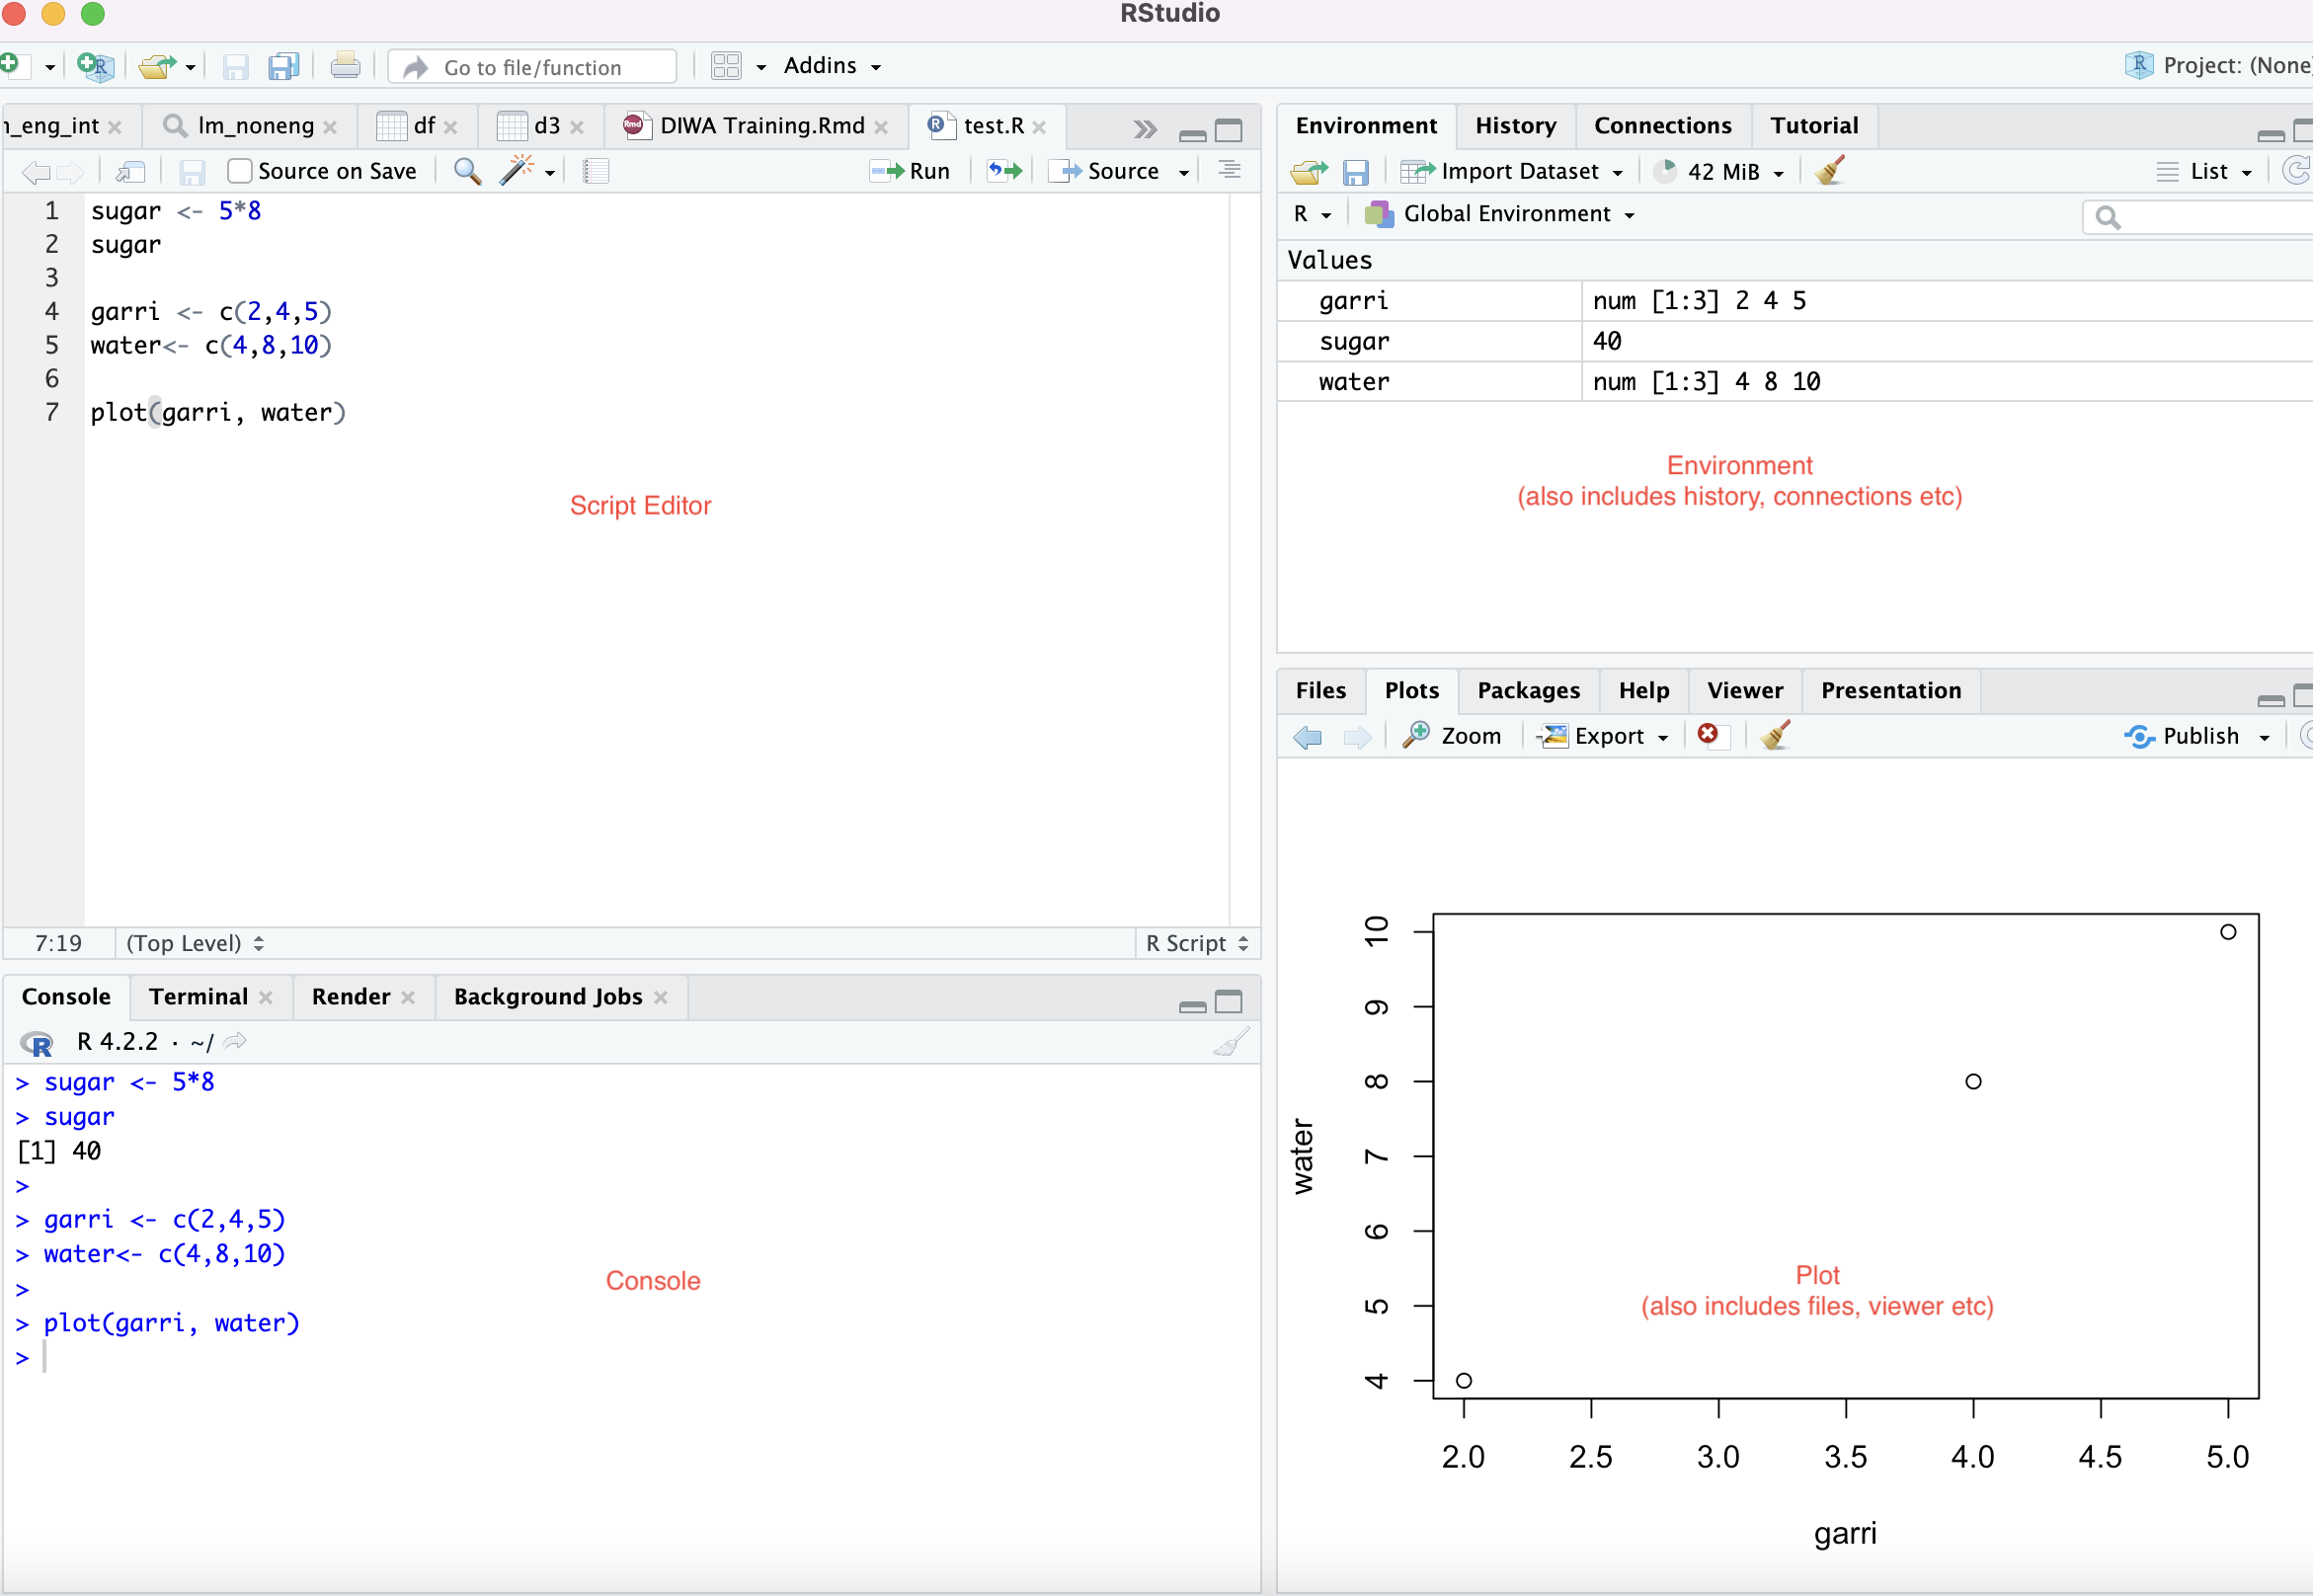
\includegraphics[width=0.9\linewidth]{4segmentsinR} \end{center}

\begin{enumerate}
\def\labelenumi{\arabic{enumi}.}
\item
  \emph{Script Editor (upper left panel):} This is where you can write
  and edit your R code. This is also where find the \texttt{run} tab or
  button needed to execute your codes.
\item
  \emph{Environment (upper right panel):} This panel has four tabs that
  includes two main tabs, Environment and History. The Environment tab
  shows information about the objects and data that you have loaded into
  R, while the History tab displays a log of the commands that you have
  executed.
\item
  \emph{Console (lower left panel):} This is where the output of your R
  code is displayed, and where you can enter commands directly.
\item
  \emph{Plot (lower right panel):} This panel includes multiple tabs,
  such as Files and Viewers, and is used to display graphics and plots
  generated by your R code.
\end{enumerate}

\hypertarget{step-2-get-to-know-your-working-directory}{%
\subsection{Step 2: Get to know your working
directory}\label{step-2-get-to-know-your-working-directory}}

\textbf{Work on the same folder (working directory) }: In R, we need to
operate within a specific folder on our system, known as the working
directory. This is where all our R code and files are stored and
accessed.

To determine your current working directory, you can use the
\texttt{getwd()} function. If it's not already present in your script
editor, simply copy the code \texttt{getwd()} and run it in your script
editor. It will display the path on your console that R is presently
utilizing. It's recommended that you keep all the files you'll be using
in R within this working directory. You may also change the working
directory if necessary, but we'll cover that later. For now, let's focus
on locating it.

\begin{Shaded}
\begin{Highlighting}[]
\FunctionTok{getwd}\NormalTok{()}
\end{Highlighting}
\end{Shaded}

\begin{verbatim}
## [1] "/Users/User3/Downloads"
\end{verbatim}

\hypertarget{step-3-understand-operators-in-r}{%
\subsection{Step 3: Understand Operators in
R}\label{step-3-understand-operators-in-r}}

\begin{itemize}
\tightlist
\item
  Assignment Operators
\item
  Arithmetic Operators
\item
  Logical Operators
\end{itemize}

\hypertarget{assignment-operators}{%
\subsubsection{Assignment Operators}\label{assignment-operators}}

\textbf{Assigning values to objects}

R stores information as an \emph{object}. You can name objects whatever
you like. Just remember to not use names that are reserved for build-in
functions or functions in the packages you use, such as sum, mean, or
abs . Most of the time, R will let you use these as names, but it leads
to confusion in your code.

Operators are used to assign values to variables, and there are two
types of assignments: leftward and rightward. The rightward assignment
operator is also commonly known as the equals \texttt{(=)} operator. For
now, we will focus on the leftward assignment operator, which is
represented by \textless-. It is called ``leftward'' because the value
on the left-hand side of the operator is assigned to the variable on the
right-hand side of the operator. The operation \textless- is often
preferred because = is used for other functions.

Operators \texttt{\textless{}-} and \texttt{=} are used to assign values
to any variable.

\begin{longtable}[]{@{}lll@{}}
\toprule\noalign{}
& Operator & Type \\
\midrule\noalign{}
\endhead
\bottomrule\noalign{}
\endlastfoot
Assignment & \textless- or = & \\
\end{longtable}

\hypertarget{few-things-to-remember}{%
\subsubsection{Few things to remember}\label{few-things-to-remember}}

\begin{itemize}
\tightlist
\item
  Do not use special characters such as \$ or \%. Common symbols that
  are used in variable names .
\item
  Remember that R is case sensitive.
\item
  The \# symbol is used for commenting and demarcation. Any code
  following \# will not be executed.
\end{itemize}

\hypertarget{arithmetic-operators}{%
\subsubsection{Arithmetic Operators}\label{arithmetic-operators}}

Just like any regular calculator, you have to pay attention to the order
of operations!

\begin{longtable}[]{@{}lll@{}}
\toprule\noalign{}
& Operator & Example \\
\midrule\noalign{}
\endhead
\bottomrule\noalign{}
\endlastfoot
Addition & + & 2+4 \\
Subtraction & - & 2-4 \\
Multiplication & * & 2*4 \\
Division & / & 4/2 \\
Exponentiation & ˆ & 2ˆ4 \\
Square Root & sqrt() & sqrt(144) \\
Absolute Value & abs() & abs(-4) \\
\end{longtable}

\hypertarget{logical-operators}{%
\subsubsection{Logical operators}\label{logical-operators}}

\begin{longtable}[]{@{}ll@{}}
\toprule\noalign{}
Operator & \\
\midrule\noalign{}
\endhead
\bottomrule\noalign{}
\endlastfoot
Less than & \textless{} \\
Less than or equal to & \textless= \\
Greater than & \textgreater{} \\
Greater than or equal to & \textgreater= \\
Exactly equal to & == (note that \texttt{=} is double) \\
Not equal to & != \\
Not x & !x \\
x or y & x y \\
x and y & x \& y! \\
\end{longtable}

Logical operators are incredibly helpful for any type of exploratory
analysis, data cleaning and/or visualization task.

\hypertarget{step-4-optional-change-your-current-working-folder}{%
\subsection{Step 4 (optional): Change your current working
folder}\label{step-4-optional-change-your-current-working-folder}}

I mentioned that we can change your current working directory (wd)
earlier. You can use the function \texttt{setwd}() to do that. You only
need to copy the path of the folder from you folder and paste it inside
the bracket.

Please \textbf{note} that in R, the separator in the path names is the
front slash \texttt{/} and not the back slash \texttt{\textbackslash{}}
that you find in most operation system . This means that if you are
copying paths directly from your operating system for this task or
future tasks, you change the path separators to front slash \texttt{/}.
The ``forward slash'' / is also more commonly used by Unix, Linux, and
macOS.

\begin{Shaded}
\begin{Highlighting}[]
\CommentTok{\#setwd("/Users/User3/Downloads")}
\end{Highlighting}
\end{Shaded}

We can also set path directly from the ``menu bar'' or ``toolbar . The
easiest way to do this is to a set default working directory: Session
\textgreater{} Set Working Directory.

\hypertarget{getting-started}{%
\section{Getting Started}\label{getting-started}}

\hypertarget{data-structures-in-r-and-executing-your-first-codes}{%
\subsection{Data Structures in R and Executing your first
codes}\label{data-structures-in-r-and-executing-your-first-codes}}

\textbf{FIND THE RUN BUTTON}: For every code you type, you need to Run
it. Please find the R button, or the button that looks like
\texttt{play} if you are using R markdown

To execute a single line of code in RStudio, you can either click the
``Run'' button at the top of the editor pane, or use the keyboard
shortcut: press Command + Return (on macOS) or Ctrl + Enter (on
Windows).

If you are working with Rmarkdown, where codes are broken down into
different chunks, you can run each chunk of code by clicking the
``play'' button next to it. Alternatively, you can use the ``Run''
dropdown and select ``Run Selected Line'' to run a specific line of
code.

To execute multiple lines of code at once, highlight the respective
portion of the code and then run it using one of the methods mentioned
above.

Now, let's start learning how to use R by exploring seven important data
structures in R:

\begin{itemize}
\tightlist
\item
  expression
\item
  object
\item
  vector
\item
  list
\item
  data frame
\item
  matrices
\item
  arrays
\end{itemize}

\begin{enumerate}
\def\labelenumi{\arabic{enumi}.}
\tightlist
\item
  \textbf{EXPRESSION}: In R, when you perform an arithmetic or logical
  operation, it is typically called a ``statement'' or an
  ``expression''. It is a special data type because in this case, you
  are not creating or modifying anything. It allows you to build simple
  or complex operations and scripts that can be executed in a single
  step.
\end{enumerate}

\begin{Shaded}
\begin{Highlighting}[]
\DecValTok{1}\SpecialCharTok{+}\DecValTok{2} \CommentTok{\# addition}
\end{Highlighting}
\end{Shaded}

\begin{verbatim}
## [1] 3
\end{verbatim}

\begin{Shaded}
\begin{Highlighting}[]
\DecValTok{8}\SpecialCharTok{/}\DecValTok{3} \CommentTok{\# division}
\end{Highlighting}
\end{Shaded}

\begin{verbatim}
## [1] 2.666667
\end{verbatim}

\begin{Shaded}
\begin{Highlighting}[]
\DecValTok{7}\SpecialCharTok{\textless{}}\DecValTok{4} \CommentTok{\# less than}
\end{Highlighting}
\end{Shaded}

\begin{verbatim}
## [1] FALSE
\end{verbatim}

\begin{Shaded}
\begin{Highlighting}[]
\DecValTok{4}\SpecialCharTok{\textgreater{}=}\DecValTok{2} \CommentTok{\#greater than or equal to}
\end{Highlighting}
\end{Shaded}

\begin{verbatim}
## [1] TRUE
\end{verbatim}

\begin{Shaded}
\begin{Highlighting}[]
\DecValTok{4} \SpecialCharTok{==} \DecValTok{4} \CommentTok{\# the same value as. Please note that \textasciigrave{}=\textasciigrave{} is double}
\end{Highlighting}
\end{Shaded}

\begin{verbatim}
## [1] TRUE
\end{verbatim}

\begin{Shaded}
\begin{Highlighting}[]
\DecValTok{4}\SpecialCharTok{!=}\DecValTok{4} \CommentTok{\# not the same value as}
\end{Highlighting}
\end{Shaded}

\begin{verbatim}
## [1] FALSE
\end{verbatim}

\begin{Shaded}
\begin{Highlighting}[]
\DecValTok{4}\SpecialCharTok{!=}\DecValTok{5} \CommentTok{\# not the same value as}
\end{Highlighting}
\end{Shaded}

\begin{verbatim}
## [1] TRUE
\end{verbatim}

\begin{Shaded}
\begin{Highlighting}[]
\FunctionTok{sqrt}\NormalTok{(}\DecValTok{144}\NormalTok{) }\CommentTok{\# square root}
\end{Highlighting}
\end{Shaded}

\begin{verbatim}
## [1] 12
\end{verbatim}

\begin{Shaded}
\begin{Highlighting}[]
\DecValTok{3}\SpecialCharTok{\^{}}\DecValTok{2}  \CommentTok{\#exponential}
\end{Highlighting}
\end{Shaded}

\begin{verbatim}
## [1] 9
\end{verbatim}

\begin{Shaded}
\begin{Highlighting}[]
\DecValTok{144}\SpecialCharTok{\^{}}\NormalTok{(}\DecValTok{1}\SpecialCharTok{/}\DecValTok{2}\NormalTok{) }\CommentTok{\# using exponential method for square root of 144}
\end{Highlighting}
\end{Shaded}

\begin{verbatim}
## [1] 12
\end{verbatim}

\begin{Shaded}
\begin{Highlighting}[]
\DecValTok{27}\SpecialCharTok{\^{}}\NormalTok{(}\DecValTok{1}\SpecialCharTok{/}\DecValTok{3}\NormalTok{) }\CommentTok{\# cube root of 27}
\end{Highlighting}
\end{Shaded}

\begin{verbatim}
## [1] 3
\end{verbatim}

\begin{enumerate}
\def\labelenumi{\arabic{enumi}.}
\setcounter{enumi}{1}
\tightlist
\item
  \textbf{OBJECT}: Since we can not do much with an expression, an
  object in R is a data structure that holds data and information. In
  order to create a new object or modify an existing one in R, we use
  the assignment operator which is represented by the symbol
  \texttt{\textless{}-} (not \texttt{\textless{}})
\end{enumerate}

\begin{Shaded}
\begin{Highlighting}[]
\NormalTok{sugar }\OtherTok{\textless{}{-}} \DecValTok{1}\SpecialCharTok{+}\DecValTok{2} \CommentTok{\# E.g 1 gram of brown sugar \& 2 grams of white sugar}
\NormalTok{garri }\OtherTok{\textless{}{-}} \DecValTok{8{-}2}  \CommentTok{\# E.g removing 2 grams of garri out of 8 grams left in a bowl}


\NormalTok{sugar }\CommentTok{\#to view  the object created, rewrite the object name}
\end{Highlighting}
\end{Shaded}

\begin{verbatim}
## [1] 3
\end{verbatim}

\begin{Shaded}
\begin{Highlighting}[]
\NormalTok{garri}
\end{Highlighting}
\end{Shaded}

\begin{verbatim}
## [1] 6
\end{verbatim}

\begin{enumerate}
\def\labelenumi{\arabic{enumi}.}
\setcounter{enumi}{2}
\tightlist
\item
  \textbf{VECTOR}: A vector is simply a list of items that are of the
  same data type. They are six types of atomic vectors- logical,
  integer, character, raw, double, and complex. A vector in R is a
  collection of elements of the same data type, such as numbers,
  characters, or logical values.
\end{enumerate}

A vector can be created by using the c() function, which concatenates
its arguments into a vector. For example, we can create the object
\texttt{sugar} and \texttt{garri} into a vector. We can also do that for
a new set of numbers. Since its not an object, it will display itself,
once you run it.

\begin{Shaded}
\begin{Highlighting}[]
\FunctionTok{c}\NormalTok{(}\StringTok{"sugar"}\NormalTok{, }\StringTok{"garri"}\NormalTok{)}
\end{Highlighting}
\end{Shaded}

\begin{verbatim}
## [1] "sugar" "garri"
\end{verbatim}

\begin{Shaded}
\begin{Highlighting}[]
\FunctionTok{c}\NormalTok{ (}\DecValTok{3}\NormalTok{,}\DecValTok{6}\NormalTok{)}
\end{Highlighting}
\end{Shaded}

\begin{verbatim}
## [1] 3 6
\end{verbatim}

\begin{enumerate}
\def\labelenumi{\arabic{enumi}.}
\setcounter{enumi}{3}
\tightlist
\item
  \textbf{LIST}: A \emph{list} in R is a data structure that can contain
  \emph{many different data types} inside it. It is ordered and
  changeable. \emph{vector} discussed above is is a collection of
  elements of the \emph{same data type} (e.g., numeric, character,
  logical) arranged in a one-dimensional array.
\end{enumerate}

A list, on the other hand, is a collection of objects of different types
(e.g., vectors, matrices, data frames, other lists) arranged in a nested
structure. In this example, you can see that we combined numeric and
character data type in the same code and created an object called
\texttt{mylist}. It is created with the built-in function \texttt{list}.

\begin{Shaded}
\begin{Highlighting}[]
\NormalTok{my\_list }\OtherTok{\textless{}{-}} \FunctionTok{list}\NormalTok{(}\FunctionTok{c}\NormalTok{(}\DecValTok{3}\NormalTok{, }\DecValTok{6}\NormalTok{, }\DecValTok{11}\NormalTok{), }\FunctionTok{c}\NormalTok{(}\StringTok{"sugar"}\NormalTok{, }\StringTok{"garri"}\NormalTok{))}
\NormalTok{my\_list}
\end{Highlighting}
\end{Shaded}

\begin{verbatim}
## [[1]]
## [1]  3  6 11
## 
## [[2]]
## [1] "sugar" "garri"
\end{verbatim}

\begin{enumerate}
\def\labelenumi{\arabic{enumi}.}
\setcounter{enumi}{4}
\tightlist
\item
  \textbf{DATA FRAMES}: The data frame is one of the most commonly used
  data structures in R, particularly for giving data a structured
  format. Data frames are represented as tables, with rows and columns
  that define the dimensions of the data. When learning R programming,
  data frames are often denoted as df, although the actual name of the
  dataset will vary - depending of the name you choose to call it . It
  is important to specify that you are creating a data frame when
  working with data in R, otherwise R may interpret it as a vector or
  list, which may not be useful for data manipulation.
\end{enumerate}

When importing external data, such as CSV or Excel files, you only need
to create an object for it. In this case, the structure of the data is
already defined in the file, so you do not need to specify it again. We
will discuss how to import data into R (such as Excel or CSV) in the
later sections. For now, we will work mainly on data (specifically
dataframes) created within R.

To create a data frame in R, you can use the data.frame() function,
which combines vectors or other data types of the same length into a
single object. Here is a simple example of how to create a data frame in
R:

\begin{Shaded}
\begin{Highlighting}[]
\NormalTok{ingredient }\OtherTok{\textless{}{-}} \FunctionTok{c}\NormalTok{(}\StringTok{"Sugar"}\NormalTok{, }\StringTok{"Garri"}\NormalTok{, }\StringTok{"Water"}\NormalTok{) }\CommentTok{\# a vector of character type}
\NormalTok{qty }\OtherTok{\textless{}{-}} \FunctionTok{c}\NormalTok{(}\DecValTok{3}\NormalTok{, }\DecValTok{6}\NormalTok{, }\DecValTok{11}\NormalTok{) }\CommentTok{\# a vector of numeric type}

\CommentTok{\# Combine vectors into a data frame}
\NormalTok{my\_df }\OtherTok{\textless{}{-}} \FunctionTok{data.frame}\NormalTok{(}\AttributeTok{Ingred =}\NormalTok{ ingredient , }\AttributeTok{Qty =}\NormalTok{ qty) }\CommentTok{\#combine them in to a df}

\CommentTok{\# View the data frame}
\NormalTok{my\_df}
\end{Highlighting}
\end{Shaded}

\begin{longtable}[]{@{}lr@{}}
\toprule\noalign{}
Ingred & Qty \\
\midrule\noalign{}
\endhead
\bottomrule\noalign{}
\endlastfoot
Sugar & 3 \\
Garri & 6 \\
Water & 11 \\
\end{longtable}

\begin{enumerate}
\def\labelenumi{\arabic{enumi}.}
\setcounter{enumi}{5}
\tightlist
\item
  \textbf{MATRICES}: We will not be needing to construct matrix and
  arrays for this lesson but it is important to know the slight
  differences between them and a data frame.
\end{enumerate}

\textbf{Difference between Matrices and Dataframe} A matrix is a two
dimensional data set with columns and rows. In a matrix, all columns and
rows must have the same length, while in a data frame, columns can have
different lengths.This means that in a data frame, each observation or
data point does not have to have the same number of variables or
features.

Overall, while matrices and data frames are both two-dimensional data
structures in R, they have different rules and properties that make them
useful for different purposes.

Matrices are best used for mathematical operations and computations,
while data frames are best used for organizing and working with
real-world data sets that may have different variable lengths and data
types.

Here is a simple example of a matrix using the \texttt{as.matrix}
function :

\begin{Shaded}
\begin{Highlighting}[]
\CommentTok{\# Create a nested list of values}
\NormalTok{my\_list }\OtherTok{\textless{}{-}} \FunctionTok{list}\NormalTok{(}\FunctionTok{c}\NormalTok{(}\DecValTok{1}\NormalTok{, }\DecValTok{3}\NormalTok{, }\DecValTok{5}\NormalTok{), }\FunctionTok{c}\NormalTok{(}\DecValTok{2}\NormalTok{, }\DecValTok{4}\NormalTok{, }\DecValTok{6}\NormalTok{))}

\CommentTok{\# Convert the list to a matrix}
\NormalTok{my\_matrix }\OtherTok{\textless{}{-}} \FunctionTok{as.matrix}\NormalTok{(my\_list)}

\CommentTok{\# Print the matrix}
\NormalTok{my\_matrix}
\end{Highlighting}
\end{Shaded}

\begin{verbatim}
##      [,1]     
## [1,] numeric,3
## [2,] numeric,3
\end{verbatim}

\begin{enumerate}
\def\labelenumi{\arabic{enumi}.}
\setcounter{enumi}{7}
\tightlist
\item
  \textbf{ARRAY} While a matrix is two-dimensiional, an array has more
  than two dimension. To understand what that means, here we create a
  3x4x3 array, where the first dimension represents the month, the
  second dimension represents the type of product (e.g., food, clothing,
  electronics), and the third dimension represents the store location
  (e.g., downtown, uptown, suburbs). Using the \texttt{array} function,
  you will see that r created another \emph{layer} for each store
  location. That means it took the two dimensions of months and
  products, and then created another dimension for each which is the
  store location. This is how arrays look like. However, we will not
  need it for this lesson as said. It is mainly used for computational
  work.
\end{enumerate}

\begin{Shaded}
\begin{Highlighting}[]
\NormalTok{sales\_data }\OtherTok{\textless{}{-}} \FunctionTok{array}\NormalTok{(}\FunctionTok{c}\NormalTok{(}\DecValTok{500}\NormalTok{, }\DecValTok{300}\NormalTok{, }\DecValTok{100}\NormalTok{, }\DecValTok{200}\NormalTok{, }\DecValTok{600}\NormalTok{, }\DecValTok{400}\NormalTok{, }\DecValTok{150}\NormalTok{, }\DecValTok{250}\NormalTok{, }\DecValTok{700}\NormalTok{, }\DecValTok{500}\NormalTok{, }\DecValTok{200}\NormalTok{, }\DecValTok{300}\NormalTok{, }\DecValTok{400}\NormalTok{, }\DecValTok{200}\NormalTok{, }\DecValTok{80}\NormalTok{, }\DecValTok{150}\NormalTok{, }\DecValTok{500}\NormalTok{, }\DecValTok{250}\NormalTok{, }\DecValTok{100}\NormalTok{, }\DecValTok{200}\NormalTok{, }\DecValTok{600}\NormalTok{, }\DecValTok{300}\NormalTok{, }\DecValTok{120}\NormalTok{, }\DecValTok{250}\NormalTok{, }\DecValTok{300}\NormalTok{, }\DecValTok{100}\NormalTok{, }\DecValTok{50}\NormalTok{, }\DecValTok{80}\NormalTok{, }\DecValTok{400}\NormalTok{, }\DecValTok{150}\NormalTok{, }\DecValTok{60}\NormalTok{, }\DecValTok{100}\NormalTok{, }\DecValTok{500}\NormalTok{, }\DecValTok{200}\NormalTok{, }\DecValTok{80}\NormalTok{, }\DecValTok{120}\NormalTok{), }\AttributeTok{dim =} \FunctionTok{c}\NormalTok{(}\DecValTok{3}\NormalTok{, }\DecValTok{4}\NormalTok{, }\DecValTok{3}\NormalTok{), }\AttributeTok{dimnames =} \FunctionTok{list}\NormalTok{(}\FunctionTok{c}\NormalTok{(}\StringTok{"Jan"}\NormalTok{, }\StringTok{"Feb"}\NormalTok{, }\StringTok{"Mar"}\NormalTok{), }\FunctionTok{c}\NormalTok{(}\StringTok{"food"}\NormalTok{, }\StringTok{"clothing"}\NormalTok{, }\StringTok{"electronics"}\NormalTok{, }\StringTok{"other"}\NormalTok{), }\FunctionTok{c}\NormalTok{(}\StringTok{"downtown"}\NormalTok{, }\StringTok{"uptown"}\NormalTok{, }\StringTok{"suburbs"}\NormalTok{)))}
\NormalTok{sales\_data}
\end{Highlighting}
\end{Shaded}

\begin{verbatim}
## , , downtown
## 
##     food clothing electronics other
## Jan  500      200         150   500
## Feb  300      600         250   200
## Mar  100      400         700   300
## 
## , , uptown
## 
##     food clothing electronics other
## Jan  400      150         100   300
## Feb  200      500         200   120
## Mar   80      250         600   250
## 
## , , suburbs
## 
##     food clothing electronics other
## Jan  300       80          60   200
## Feb  100      400         100    80
## Mar   50      150         500   120
\end{verbatim}

\hypertarget{basic-terms-in-r}{%
\subsection{Basic Terms in R}\label{basic-terms-in-r}}

\begin{itemize}
\item
  \textbf{Functions}: is a block of organized and reusable code that
  performs a specific tasks which are often inbuilt. Additionally, users
  can also create new in a customized function There are many in-built
  functions in R but a simple example is the mean which is referred to
  as\texttt{mean()}. The mean of a vector of nuber called \texttt{x}
  will be \texttt{mean(x)}.
\item
  \textbf{Parameters}: are passed into a function as inputs to modify
  the result. For example,to tell R to ignore missing values while
  computing the means, you can use the paramater \texttt{na.rm=TRUE}
  that inside the \texttt{mean()} function. This will be written as
  \texttt{mean(x,\ na.rm=\ TRUE)}. The \texttt{na.rm=TRUE} is the
  parameter.
\item
  \textbf{Help and Documentation}: if you need help on knowing the
  parameters in a function or more information about any function, you
  can use the help function which is denoted as \texttt{help()} or
  \texttt{?()}. For the mean function, for example, the code for help or
  its documentation will be \texttt{help(mean)} or \texttt{?mean}.
\item
  \textbf{Packages \& library}: Base R, the default installation of R,
  does not include certain tools. However, other authors have created
  these tools, which can be imported into R by following two procedures.
  First, you must install them, which is a one-time process, and these
  tools are known as packages. Once installed, you must inform R that
  you want to use a specific package by calling the \texttt{library}
  function whenever you need to use the tools included in that package.
\end{itemize}

\hypertarget{basic-functions-in-r}{%
\subsection{Basic Functions in R}\label{basic-functions-in-r}}

\begin{itemize}
\item
  str(): returns the data types of each column in a dataframe.
\item
  head(): often used do display the first nth rows (observation) of a
  dataframe, rather all the rows, especially for larger datasets. The
  default n is 6, but you can specify the n.
\item
  tail(): just like the head, often used do display the last few rows
  (observations) of a dataframe, rather all the rows, especially for
  larger datasets. The default n is 6, but you can specify the n.
\item
  nrow(): returns the number of rows (observations) in the dataset.
\item
  ncol(): returns the number of columns (variables) in the datasets.
\item
  colnames() : returns the column names.
\item
  rownames(): returns the row names.
\item
  dim(): returns the number row and columns together (referred to as
  dimension). It returns a vector of length two with the number of rows
  in the first element and the number of columns in the second element.
\item
  unique() : returns unique observations only.
\item
  class(): It returns a character vector that describes the class or
  classes of the object.
\end{itemize}

\hypertarget{examples-of-basic-functions-in-r}{%
\subsubsection{Examples of Basic Functions in
R}\label{examples-of-basic-functions-in-r}}

\begin{Shaded}
\begin{Highlighting}[]
\FunctionTok{str}\NormalTok{(my\_df)}
\end{Highlighting}
\end{Shaded}

\begin{verbatim}
## 'data.frame':    3 obs. of  2 variables:
##  $ Ingred: chr  "Sugar" "Garri" "Water"
##  $ Qty   : num  3 6 11
\end{verbatim}

\begin{Shaded}
\begin{Highlighting}[]
\CommentTok{\# Show the first "n" rows (default is 6)}
\FunctionTok{head}\NormalTok{(my\_df, }\AttributeTok{n =} \DecValTok{2}\NormalTok{)}
\end{Highlighting}
\end{Shaded}

\begin{longtable}[]{@{}lr@{}}
\toprule\noalign{}
Ingred & Qty \\
\midrule\noalign{}
\endhead
\bottomrule\noalign{}
\endlastfoot
Sugar & 3 \\
Garri & 6 \\
\end{longtable}

\begin{Shaded}
\begin{Highlighting}[]
\CommentTok{\# Show the last "n" rows (default is 6)}
\FunctionTok{tail}\NormalTok{(my\_df, }\AttributeTok{n =} \DecValTok{2}\NormalTok{)}
\end{Highlighting}
\end{Shaded}

\begin{longtable}[]{@{}llr@{}}
\toprule\noalign{}
& Ingred & Qty \\
\midrule\noalign{}
\endhead
\bottomrule\noalign{}
\endlastfoot
2 & Garri & 6 \\
3 & Water & 11 \\
\end{longtable}

\begin{Shaded}
\begin{Highlighting}[]
\CommentTok{\# Dimensions of dataframe}
\FunctionTok{dim}\NormalTok{(my\_df)}
\end{Highlighting}
\end{Shaded}

\begin{verbatim}
## [1] 3 2
\end{verbatim}

\begin{Shaded}
\begin{Highlighting}[]
\CommentTok{\# Number of rows}
\FunctionTok{nrow}\NormalTok{(my\_df)}
\end{Highlighting}
\end{Shaded}

\begin{verbatim}
## [1] 3
\end{verbatim}

\begin{Shaded}
\begin{Highlighting}[]
\CommentTok{\# Number of cols}
\FunctionTok{ncol}\NormalTok{(my\_df)}
\end{Highlighting}
\end{Shaded}

\begin{verbatim}
## [1] 2
\end{verbatim}

\begin{Shaded}
\begin{Highlighting}[]
\CommentTok{\# Show column names (two different ways)}
\FunctionTok{colnames}\NormalTok{(my\_df)}
\end{Highlighting}
\end{Shaded}

\begin{verbatim}
## [1] "Ingred" "Qty"
\end{verbatim}

\begin{Shaded}
\begin{Highlighting}[]
\FunctionTok{names}\NormalTok{(my\_df) }
\end{Highlighting}
\end{Shaded}

\begin{verbatim}
## [1] "Ingred" "Qty"
\end{verbatim}

\begin{Shaded}
\begin{Highlighting}[]
\CommentTok{\# Show row names (unnamed: default to character type for row number)}
\FunctionTok{rownames}\NormalTok{(my\_df)}
\end{Highlighting}
\end{Shaded}

\begin{verbatim}
## [1] "1" "2" "3"
\end{verbatim}

\begin{Shaded}
\begin{Highlighting}[]
\CommentTok{\# Show rows with unique data}
\FunctionTok{unique}\NormalTok{(my\_df)}
\end{Highlighting}
\end{Shaded}

\begin{longtable}[]{@{}lr@{}}
\toprule\noalign{}
Ingred & Qty \\
\midrule\noalign{}
\endhead
\bottomrule\noalign{}
\endlastfoot
Sugar & 3 \\
Garri & 6 \\
Water & 11 \\
\end{longtable}

\begin{Shaded}
\begin{Highlighting}[]
\CommentTok{\# install a package:}

\CommentTok{\# call an installed package }
\FunctionTok{library}\NormalTok{ (dplyr)}
\end{Highlighting}
\end{Shaded}

\hypertarget{data-manipulation-in-base-r}{%
\section{Data Manipulation in Base
R}\label{data-manipulation-in-base-r}}

``Base R'' is the term used to describe the fundamental set of functions
and data structures that come pre-installed with the R programming
language. These functions and structures serve as the building blocks
for all R code. To demonstrate the use of Base R, let's create our first
dataset and manipulate the data with these core functions.

\hypertarget{my-first-dataset-in-r}{%
\subsection{My first dataset in R}\label{my-first-dataset-in-r}}

As the research manager of a multinational organization, you have
received complaints of weight discrimination against overweight women
(assumed here to mean those weighing 100kg and above) during the hiring
process, even though a policy prohibiting such discrimination has been
in place since 2015. To investigate this issue further, you have
randomly selected a sample of 20 staff members and recorded their
weights. Your sample is evenly split between men and women, with 10
individuals of each gender.

The men's weights (in kg) are (89, 75, 88, 75, 49, 89, 110, 120, 89, and
75), while the women's weights (in kg) are (75, 76, 87, 110, 67, 76, 43,
55, 59, and 60). You also collected additional information about the
sample staff. Here we want to create a dataset of 6 variables consisting
data about 20 staff in the organization. The variables are
\texttt{Gender}, \texttt{Weight}, \texttt{income}, \texttt{rating},
\texttt{marital\ status} and whether staff stays in the
\texttt{city\ central}.

\begin{itemize}
\tightlist
\item
  \textbf{Gender}: is to know whether they considered to be male or
  female
\item
  \textbf{Weight} is their human body weight measured in kiloggram
\item
  \textbf{Income}: Their monthly income in dollars
\item
  \textbf{rating}: Their rating of the recruitment process
\item
  \textbf{Marstatus}: is whether they are single, married or divorced
\item
  \textbf{CityCentral}: is whether they stay close to the city central
  or not
\end{itemize}

\begin{Shaded}
\begin{Highlighting}[]
\CommentTok{\# Create Gender variable and ensure to enclose characters in quotes.}

\NormalTok{Gender }\OtherTok{\textless{}{-}} \FunctionTok{c}\NormalTok{(}\StringTok{"Male"}\NormalTok{, }\StringTok{"Male"}\NormalTok{, }\StringTok{"Male"}\NormalTok{, }\StringTok{"Male"}\NormalTok{, }\StringTok{"Male"}\NormalTok{, }
            \StringTok{"Male"}\NormalTok{, }\StringTok{"Male"}\NormalTok{, }\StringTok{"Male"}\NormalTok{, }\StringTok{"Male"}\NormalTok{, }\StringTok{"Male"}\NormalTok{, }
            \StringTok{"FeMale"}\NormalTok{,}\StringTok{"FeMale"}\NormalTok{, }\StringTok{"FeMale"}\NormalTok{,}\StringTok{"FeMale"}\NormalTok{, }\StringTok{"FeMale"}\NormalTok{,}
           \StringTok{"FeMale"}\NormalTok{,}\StringTok{"FeMale"}\NormalTok{,}\StringTok{"FeMale"}\NormalTok{,}\StringTok{"FeMale"}\NormalTok{,}\StringTok{"FeMale"}\NormalTok{)}

\CommentTok{\#another method for creating the same Gender variable  is using the \textasciigrave{}rep\textasciigrave{} function}
\CommentTok{\# Gender \textless{}{-} c(rep("Male", 10), rep("Female", 10))}

\CommentTok{\# create weight}
\NormalTok{weight }\OtherTok{\textless{}{-}} \FunctionTok{c}\NormalTok{(}\DecValTok{89}\NormalTok{, }\DecValTok{75}\NormalTok{, }\DecValTok{88}\NormalTok{, }\DecValTok{75}\NormalTok{, }\DecValTok{49}\NormalTok{, }\DecValTok{89}\NormalTok{, }\DecValTok{110}\NormalTok{, }\DecValTok{120}\NormalTok{, }\DecValTok{89}\NormalTok{, }\DecValTok{75}\NormalTok{, }
            \DecValTok{75}\NormalTok{, }\DecValTok{76}\NormalTok{, }\DecValTok{87}\NormalTok{, }\DecValTok{110}\NormalTok{, }\DecValTok{67}\NormalTok{, }\DecValTok{76}\NormalTok{, }\DecValTok{43}\NormalTok{, }\DecValTok{55}\NormalTok{, }\DecValTok{59}\NormalTok{, }\DecValTok{60}\NormalTok{) }

\CommentTok{\# create income}
\NormalTok{income }\OtherTok{\textless{}{-}} \FunctionTok{c}\NormalTok{(}\DecValTok{50000}\NormalTok{, }\DecValTok{95000}\NormalTok{, }\DecValTok{120000}\NormalTok{, }\DecValTok{800000}\NormalTok{, }\DecValTok{650000}\NormalTok{, }\DecValTok{92000}\NormalTok{, }\DecValTok{94000}\NormalTok{, }\DecValTok{222000}\NormalTok{, }\DecValTok{543000}\NormalTok{,}\DecValTok{75000}\NormalTok{,}
            \DecValTok{63000}\NormalTok{, }\DecValTok{40000}\NormalTok{, }\DecValTok{99000}\NormalTok{, }\DecValTok{450000}\NormalTok{, }\DecValTok{180000}\NormalTok{, }\DecValTok{190000}\NormalTok{, }\DecValTok{96000}\NormalTok{, }\DecValTok{780000}\NormalTok{, }\DecValTok{150000}\NormalTok{, }\DecValTok{342000}\NormalTok{)}

\CommentTok{\# create weight}
\NormalTok{rating }\OtherTok{\textless{}{-}} \FunctionTok{c}\NormalTok{(}\DecValTok{5}\NormalTok{, }\DecValTok{1}\NormalTok{, }\DecValTok{2}\NormalTok{, }\DecValTok{4}\NormalTok{, }\DecValTok{9}\NormalTok{, }\DecValTok{9}\NormalTok{, }\DecValTok{8}\NormalTok{, }\DecValTok{1}\NormalTok{, }\DecValTok{9}\NormalTok{, }\DecValTok{7}\NormalTok{, }
            \DecValTok{5}\NormalTok{, }\DecValTok{6}\NormalTok{, }\DecValTok{6}\NormalTok{, }\DecValTok{1}\NormalTok{, }\DecValTok{1}\NormalTok{, }\DecValTok{1}\NormalTok{, }\DecValTok{3}\NormalTok{, }\DecValTok{6}\NormalTok{, }\DecValTok{9}\NormalTok{, }\DecValTok{4}\NormalTok{) }

\NormalTok{Marstatus }\OtherTok{\textless{}{-}} \FunctionTok{c}\NormalTok{(}\StringTok{"Married"}\NormalTok{, }\StringTok{"Married"}\NormalTok{,}\StringTok{"Single"}\NormalTok{, }\StringTok{"Single"}\NormalTok{,}\StringTok{"Single"}\NormalTok{,}
             \StringTok{"Single"}\NormalTok{, }\StringTok{"Divorced"}\NormalTok{,}\StringTok{"Single"}\NormalTok{, }\StringTok{"Married"}\NormalTok{,}\StringTok{"Single"}\NormalTok{,}
             \StringTok{"Married"}\NormalTok{, }\StringTok{"Single"}\NormalTok{,}\StringTok{"Single"}\NormalTok{, }\StringTok{"Divorced"}\NormalTok{,}\StringTok{"Single"}\NormalTok{,}
             \StringTok{"Single"}\NormalTok{, }\StringTok{"Divorced"}\NormalTok{, }\StringTok{"Single"}\NormalTok{,}\StringTok{"Married"}\NormalTok{, }\StringTok{"Divorced"}\NormalTok{)}

\NormalTok{CityCentral }\OtherTok{\textless{}{-}} \FunctionTok{c}\NormalTok{(}\StringTok{"Yes"}\NormalTok{,}\StringTok{"No"}\NormalTok{,}\StringTok{"Yes"}\NormalTok{,}\StringTok{"Yes"}\NormalTok{,}\StringTok{"Yes"}\NormalTok{,}\StringTok{"Yes"}\NormalTok{,}\StringTok{"Yes"}\NormalTok{,}\StringTok{"Yes"}\NormalTok{,}\StringTok{"No"}\NormalTok{,}\StringTok{"Yes"}\NormalTok{,}
                 \StringTok{"No"}\NormalTok{,}\StringTok{"No"}\NormalTok{,}\StringTok{"Yes"}\NormalTok{,}\StringTok{"Yes"}\NormalTok{,}\StringTok{"No"}\NormalTok{,}\StringTok{"Yes"}\NormalTok{,}\StringTok{"No"}\NormalTok{,}\StringTok{"Yes"}\NormalTok{,}\StringTok{"No"}\NormalTok{,}\StringTok{"No"}\NormalTok{)}


\CommentTok{\#Create a dataframe, method 1: A simplier method using the \textasciigrave{}data.frame\textasciigrave{} function }
\NormalTok{officew }\OtherTok{\textless{}{-}} \FunctionTok{data.frame}\NormalTok{(Gender, weight, income, rating, Marstatus, }
\NormalTok{                               CityCentral)}

\CommentTok{\# Create a dataframe. method 2:  In the method below you have to use  cbind and \textasciigrave{}as.data.frame\textasciigrave{} function . Not the most efficient method.}

\CommentTok{\#officew \textless{}{-} as.data.frame(cbind(Gender, weight, income, rating, Marstatus, }
                           \CommentTok{\#    CityCentral))}

\NormalTok{officew }
\end{Highlighting}
\end{Shaded}

\begin{longtable}[]{@{}lrrrll@{}}
\toprule\noalign{}
Gender & weight & income & rating & Marstatus & CityCentral \\
\midrule\noalign{}
\endhead
\bottomrule\noalign{}
\endlastfoot
Male & 89 & 50000 & 5 & Married & Yes \\
Male & 75 & 95000 & 1 & Married & No \\
Male & 88 & 120000 & 2 & Single & Yes \\
Male & 75 & 800000 & 4 & Single & Yes \\
Male & 49 & 650000 & 9 & Single & Yes \\
Male & 89 & 92000 & 9 & Single & Yes \\
Male & 110 & 94000 & 8 & Divorced & Yes \\
Male & 120 & 222000 & 1 & Single & Yes \\
Male & 89 & 543000 & 9 & Married & No \\
Male & 75 & 75000 & 7 & Single & Yes \\
FeMale & 75 & 63000 & 5 & Married & No \\
FeMale & 76 & 40000 & 6 & Single & No \\
FeMale & 87 & 99000 & 6 & Single & Yes \\
FeMale & 110 & 450000 & 1 & Divorced & Yes \\
FeMale & 67 & 180000 & 1 & Single & No \\
FeMale & 76 & 190000 & 1 & Single & Yes \\
FeMale & 43 & 96000 & 3 & Divorced & No \\
FeMale & 55 & 780000 & 6 & Single & Yes \\
FeMale & 59 & 150000 & 9 & Married & No \\
FeMale & 60 & 342000 & 4 & Divorced & No \\
\end{longtable}

You will notice that when were creating new vectors we used the
\texttt{c()} function which is used to concatenate or combine different
elements into a single object.

It will good to note that R assumes that each observation in a variable
corresponds to the same individual across all other variables. For
example, the first observation in the \texttt{Gender} variable is
assumed to be the same person as the first observation in the
\texttt{Income} variable, who earns 50,000, has a rating of 5, and is
married. Therefore, it is essential to maintain the order of
observations across variables.

Additionally, we can also use the cbind() function to combine multiple
objects as columns into a single data frame object in R. We will explain
this in more detail later on. However, I paused that method since its
inefficient.

\hypertarget{lets-do-some-basic-stats}{%
\subsection{Let's do some BASIC STATS}\label{lets-do-some-basic-stats}}

\hypertarget{the-mean-sd-mode-median}{%
\subsection{The Mean, SD, Mode, Median}\label{the-mean-sd-mode-median}}

\begin{Shaded}
\begin{Highlighting}[]
\FunctionTok{mean}\NormalTok{(officew}\SpecialCharTok{$}\NormalTok{income, }\AttributeTok{na.rm=}\NormalTok{T)}
\end{Highlighting}
\end{Shaded}

\begin{verbatim}
## [1] 256550
\end{verbatim}

\begin{Shaded}
\begin{Highlighting}[]
\FunctionTok{sd}\NormalTok{(officew}\SpecialCharTok{$}\NormalTok{income, }\AttributeTok{na.rm=}\NormalTok{T)}
\end{Highlighting}
\end{Shaded}

\begin{verbatim}
## [1] 249481
\end{verbatim}

\begin{Shaded}
\begin{Highlighting}[]
\FunctionTok{mean}\NormalTok{(officew}\SpecialCharTok{$}\NormalTok{weight, }\AttributeTok{na.rm=}\NormalTok{T)}
\end{Highlighting}
\end{Shaded}

\begin{verbatim}
## [1] 78.35
\end{verbatim}

\begin{Shaded}
\begin{Highlighting}[]
\FunctionTok{sd}\NormalTok{(officew}\SpecialCharTok{$}\NormalTok{weight, }\AttributeTok{na.rm=}\NormalTok{T)}
\end{Highlighting}
\end{Shaded}

\begin{verbatim}
## [1] 20.25957
\end{verbatim}

\begin{Shaded}
\begin{Highlighting}[]
\FunctionTok{mode}\NormalTok{(officew}\SpecialCharTok{$}\NormalTok{rating)}
\end{Highlighting}
\end{Shaded}

\begin{verbatim}
## [1] "numeric"
\end{verbatim}

\begin{Shaded}
\begin{Highlighting}[]
\FunctionTok{median}\NormalTok{(officew}\SpecialCharTok{$}\NormalTok{rating)}
\end{Highlighting}
\end{Shaded}

\begin{verbatim}
## [1] 5
\end{verbatim}

\hypertarget{converting-a-character-into-a-factor}{%
\subsubsection{Converting a character into a
factor}\label{converting-a-character-into-a-factor}}

First, you want to check the class (data type) of the variable

\begin{Shaded}
\begin{Highlighting}[]
\FunctionTok{class}\NormalTok{(officew}\SpecialCharTok{$}\NormalTok{Marstatus)}
\end{Highlighting}
\end{Shaded}

\begin{verbatim}
## [1] "character"
\end{verbatim}

As you may remember, it was created as a character variable and most
times, we want marital status to be a categorical variable. You will use
\texttt{as.factor()} function, \texttt{factor()} or
\texttt{as.factor(as.character())} referred in nested approch to perform
this operation. For simplicity, I advise you use \texttt{as.factor()}

\begin{Shaded}
\begin{Highlighting}[]
\NormalTok{officew}\SpecialCharTok{$}\NormalTok{Marstatus}\OtherTok{\textless{}{-}} \FunctionTok{as.factor}\NormalTok{(officew}\SpecialCharTok{$}\NormalTok{Marstatus)}
\CommentTok{\#officew$Marstatus\textless{}{-} as.factor(as.character(officew$Marstatus))}

\FunctionTok{class}\NormalTok{(officew}\SpecialCharTok{$}\NormalTok{income)}
\end{Highlighting}
\end{Shaded}

\begin{verbatim}
## [1] "numeric"
\end{verbatim}

To create a Marital status variable in R, the most efficient way is to
use the \texttt{factor()} function and specify the levels using the
levels argument. This eliminates the need to convert the variable from
character to numeric later on.

This creates a factor variable with the specified levels and assigns it
to the object \texttt{Marstatus}. This approach can save time and reduce
errors in your code.

\begin{Shaded}
\begin{Highlighting}[]
\CommentTok{\# Define the levels of the factor}
\NormalTok{marital\_levels }\OtherTok{\textless{}{-}} \FunctionTok{c}\NormalTok{(}\StringTok{"Single"}\NormalTok{, }\StringTok{"Married"}\NormalTok{, }\StringTok{"Divorced"}\NormalTok{)}

\CommentTok{\# Create the factor variable with specified levels}
\NormalTok{Marstatus }\OtherTok{\textless{}{-}} \FunctionTok{factor}\NormalTok{(}\FunctionTok{c}\NormalTok{(}\StringTok{"Married"}\NormalTok{, }\StringTok{"Married"}\NormalTok{, }\StringTok{"Single"}\NormalTok{, }\StringTok{"Single"}\NormalTok{, }\StringTok{"Single"}\NormalTok{, }\StringTok{"Single"}\NormalTok{, }\StringTok{"Divorced"}\NormalTok{, }\StringTok{"Single"}\NormalTok{, }\StringTok{"Married"}\NormalTok{, }\StringTok{"Single"}\NormalTok{, }\StringTok{"Married"}\NormalTok{, }\StringTok{"Single"}\NormalTok{, }\StringTok{"Single"}\NormalTok{, }\StringTok{"Divorced"}\NormalTok{, }\StringTok{"Single"}\NormalTok{, }\StringTok{"Single"}\NormalTok{, }\StringTok{"Divorced"}\NormalTok{, }\StringTok{"Single"}\NormalTok{, }\StringTok{"Married"}\NormalTok{, }\StringTok{"Divorced"}\NormalTok{), }\AttributeTok{levels =}\NormalTok{ marital\_levels)}

\CommentTok{\# View the levels and values of the factor}
\FunctionTok{levels}\NormalTok{(Marstatus)}
\end{Highlighting}
\end{Shaded}

\begin{verbatim}
## [1] "Single"   "Married"  "Divorced"
\end{verbatim}

\hypertarget{importing-files}{%
\subsection{Importing files}\label{importing-files}}

\hypertarget{direct-importing}{%
\subsubsection{Direct Importing}\label{direct-importing}}

R allows you to import data from a variety of file formats, including
\texttt{csv}, \texttt{xls}, \texttt{dta} (Stata), and \texttt{sav}
(SPSS) files. To import data, you first need to load the required
libraries and then use the appropriate function for the file format.

For example, if you have a \texttt{dta} file and want to import it into
R, you can use the \texttt{readr()} library and the \texttt{read\_dta}
function inside the library. Alternatively, if you have a \texttt{csv}
file, you can use the read\_csv function from the same library.

\begin{Shaded}
\begin{Highlighting}[]
\FunctionTok{library}\NormalTok{(readr)}
\NormalTok{officew\_1 }\OtherTok{\textless{}{-}} \FunctionTok{read\_csv}\NormalTok{(}\StringTok{"officew.csv"}\NormalTok{)}
\end{Highlighting}
\end{Shaded}

This code loads the \texttt{readr} library, reads the \texttt{dta} file
located at \texttt{/officew.csv}, and assigns the resulting data to the
\texttt{officew\_1} object. The file must have been located in your
working directory.

\hypertarget{specifying-parameters-when-importing}{%
\subsubsection{Specifying parameters when
importing}\label{specifying-parameters-when-importing}}

\begin{Shaded}
\begin{Highlighting}[]
\FunctionTok{library}\NormalTok{(readr)}
\NormalTok{officew\_2 }\OtherTok{\textless{}{-}}\FunctionTok{read.table}\NormalTok{(}\StringTok{"officew.csv"}\NormalTok{,}
         \AttributeTok{header=}\ConstantTok{FALSE}\NormalTok{, }\CommentTok{\# change to "TRUE" to retain the header (column names)}
          \AttributeTok{sep=}\StringTok{","}         \CommentTok{\# use "\textbackslash{}t" for tab{-}delimited files}
\NormalTok{)}
\end{Highlighting}
\end{Shaded}

By default, when importing data into R, character variables are
converted to factors. However, this may not always be desirable, and you
may want to treat some of these variables as character strings instead.
To do this, you can use the \texttt{stringsAsFactors} argument when
importing data and set it to \texttt{FALSE}.

For example, if you have a csv file with character variables and want to
import it into R without converting them to factors, you can use the
read\_csv() function from the readr library and set
\texttt{stringsAsFactors\ =\ FALSE} as shown below:

\begin{Shaded}
\begin{Highlighting}[]
\NormalTok{officew\_4 }\OtherTok{\textless{}{-}} \FunctionTok{read.csv}\NormalTok{(}\StringTok{"officew.csv"}\NormalTok{, }\AttributeTok{stringsAsFactors=}\ConstantTok{FALSE}\NormalTok{)}
\NormalTok{officew\_5 }\OtherTok{\textless{}{-}} \FunctionTok{read.csv}\NormalTok{(}\StringTok{"officew.csv"}\NormalTok{, }\AttributeTok{stringsAsFactors=}\ConstantTok{TRUE}\NormalTok{)}
\FunctionTok{str}\NormalTok{(officew\_4)}
\end{Highlighting}
\end{Shaded}

\begin{verbatim}
## 'data.frame':    20 obs. of  7 variables:
##  $ X          : int  1 2 3 4 5 6 7 8 9 10 ...
##  $ Gender     : chr  "Male" "Male" "Male" "Male" ...
##  $ weight     : int  89 75 88 75 49 89 110 120 89 75 ...
##  $ income     : num  50000 95000 120000 800000 650000 92000 94000 222000 543000 75000 ...
##  $ rating     : int  5 1 2 4 9 9 8 1 9 7 ...
##  $ Marstatus  : chr  "Married" "Married" "Single" "Single" ...
##  $ CityCentral: chr  "Yes" "No" "Yes" "Yes" ...
\end{verbatim}

\begin{Shaded}
\begin{Highlighting}[]
\FunctionTok{str}\NormalTok{(officew\_5)}
\end{Highlighting}
\end{Shaded}

\begin{verbatim}
## 'data.frame':    20 obs. of  7 variables:
##  $ X          : int  1 2 3 4 5 6 7 8 9 10 ...
##  $ Gender     : Factor w/ 2 levels "FeMale","Male": 2 2 2 2 2 2 2 2 2 2 ...
##  $ weight     : int  89 75 88 75 49 89 110 120 89 75 ...
##  $ income     : num  50000 95000 120000 800000 650000 92000 94000 222000 543000 75000 ...
##  $ rating     : int  5 1 2 4 9 9 8 1 9 7 ...
##  $ Marstatus  : Factor w/ 3 levels "Divorced","Married",..: 2 2 3 3 3 3 1 3 2 3 ...
##  $ CityCentral: Factor w/ 2 levels "No","Yes": 2 1 2 2 2 2 2 2 1 2 ...
\end{verbatim}

Conversely, if you want all character variables to be converted to
factors, you can set \texttt{stringsAsFactors\ =\ TRUE}. However, note
that this may not be appropriate for all datasets, and you should
carefully consider the implications before making this choice.

\hypertarget{importing-files-from-github}{%
\subsubsection{Importing files from
Github}\label{importing-files-from-github}}

If you have data stored in the cloud such as github, you can use read
\texttt{getURL} function in the \texttt{RCurl} library to import it from
the cloud into R, and then read it with your preferred format such as
\texttt{dta}. Please note that importing from using \texttt{Rcurl}
usually requires two steps. The first is getting it from the cloud and
the importing it into R in a format that can be used.

\begin{Shaded}
\begin{Highlighting}[]
\CommentTok{\#install.packages("readr")}
\CommentTok{\#library(readxl)}

\FunctionTok{library}\NormalTok{(openxlsx)}\CommentTok{\# export to excel}
\FunctionTok{library}\NormalTok{(RCurl)}
\NormalTok{x }\OtherTok{\textless{}{-}} \FunctionTok{getURL}\NormalTok{(}\StringTok{"https://raw.githubusercontent.com/abiola1864/FLS301/main/officew.csv"}\NormalTok{)}
\NormalTok{officew}\OtherTok{\textless{}{-}} \FunctionTok{read.csv}\NormalTok{(}\AttributeTok{text =}\NormalTok{ x)}
\FunctionTok{head}\NormalTok{(officew)}
\end{Highlighting}
\end{Shaded}

\begin{longtable}[]{@{}rlrrrll@{}}
\toprule\noalign{}
X & Gender & weight & income & rating & Marstatus & CityCentral \\
\midrule\noalign{}
\endhead
\bottomrule\noalign{}
\endlastfoot
1 & Male & 89 & 50000 & 5 & Married & Yes \\
2 & Male & 75 & 95000 & 1 & Married & No \\
3 & Male & 88 & 120000 & 2 & Single & Yes \\
4 & Male & 75 & 800000 & 4 & Single & Yes \\
5 & Male & 49 & 650000 & 9 & Single & Yes \\
6 & Male & 89 & 92000 & 9 & Single & Yes \\
\end{longtable}

You can also just import it directly using \texttt{read.csv} if its a
.csv file.

\begin{Shaded}
\begin{Highlighting}[]
\NormalTok{x1 }\OtherTok{\textless{}{-}} \FunctionTok{read.csv}\NormalTok{(}\StringTok{"https://raw.githubusercontent.com/abiola1864/FLS301/main/officew.csv"}\NormalTok{)}
\end{Highlighting}
\end{Shaded}

\hypertarget{exporting-files-from-r}{%
\subsection{Exporting files from R}\label{exporting-files-from-r}}

To export data from R, you can use the \texttt{write.csv()} or
\texttt{write\_sav()} functions to save your data as a csv or SPSS file,
respectively. Other export options are also available depending on the
format you need.

For example, to export your data as a csv file, you can use the
\texttt{write.csv()} function and specify the name of the file and the
data object you want to export. Similarly, to export your data as an
SPSS file, you can use the haven package and the \texttt{write\_sav()}
function:

\begin{Shaded}
\begin{Highlighting}[]
\FunctionTok{library}\NormalTok{(openxlsx)}\CommentTok{\# export to excel}
\FunctionTok{library}\NormalTok{(haven)}

\FunctionTok{write.csv}\NormalTok{(officew, }\StringTok{"officew.csv"}\NormalTok{) }\CommentTok{\#export to csv}
\FunctionTok{write\_sav}\NormalTok{(officew, }\StringTok{"officew.sav"}\NormalTok{)}\CommentTok{\#export to spss}
\end{Highlighting}
\end{Shaded}

\hypertarget{subsetting}{%
\section{Subsetting}\label{subsetting}}

There are multiple approaches to extract a subset of data from a larger
data frame in R. One popular method is to utilize the \texttt{select} or
\texttt{filter} function from the dplyr package, which we will cover
later. These functions enable the extraction of specific columns of
data, such as selecting only the female Gender respondents.

Another method is to use the index position or the \texttt{subset}
function to extract rows that meet certain criteria, such as only
including data for females. In this section, we will focus on the second
method. This can be accomplished in two ways, either by referring to the
variable name or the index position in R.

Index subsetting in R is performed using the bracket notation with
indices for rows or columns. For instance, df{[}row\_index,
column\_index{]} returns the specified rows and columns.

If you want the first row, use df{[}1, {]}, while df{[}, 1{]} or
df{[}1{]} returns the first column. Note that the comma's position
changes based on whether you want to return rows or columns. To focus on
rows, place a comma after the index and leave the column index blank,
e.g., df{[}1, {]} returns the first row, whereas df{[}, 1 {]} or
df{[}1{]} with no comma returns the first column. Likewise, df{[}c(1,
2), {]} returns the first and second rows, and df{[}, c(1, 2){]} returns
the first and second columns.

\hypertarget{subsetting-in-base-r-by-variable-name}{%
\subsection{Subsetting in Base R by Variable
Name}\label{subsetting-in-base-r-by-variable-name}}

\begin{Shaded}
\begin{Highlighting}[]
\CommentTok{\# subset female gender}
\NormalTok{officew\_women1 }\OtherTok{\textless{}{-}}\NormalTok{ officew[officew}\SpecialCharTok{$}\NormalTok{Gender }\SpecialCharTok{==} \StringTok{"FeMale"}\NormalTok{,]}

\CommentTok{\# subset female gender , another method}
\NormalTok{officew\_women2 }\OtherTok{\textless{}{-}} \FunctionTok{subset}\NormalTok{(officew, Gender }\SpecialCharTok{==} \StringTok{"FeMale"}\NormalTok{)}

\CommentTok{\# subset female gender and weight}
\NormalTok{officew\_women3 }\OtherTok{\textless{}{-}} \FunctionTok{subset}\NormalTok{(officew, Gender }\SpecialCharTok{==} \StringTok{"FeMale"}\NormalTok{, }\AttributeTok{select =} 
                           \FunctionTok{c}\NormalTok{(}\StringTok{"weight"}\NormalTok{))}



\FunctionTok{head}\NormalTok{(officew\_women2[, }\DecValTok{1}\SpecialCharTok{:}\DecValTok{5}\NormalTok{])}
\end{Highlighting}
\end{Shaded}

\begin{longtable}[]{@{}lrlrrr@{}}
\toprule\noalign{}
& X & Gender & weight & income & rating \\
\midrule\noalign{}
\endhead
\bottomrule\noalign{}
\endlastfoot
11 & 11 & FeMale & 75 & 63000 & 5 \\
12 & 12 & FeMale & 76 & 40000 & 6 \\
13 & 13 & FeMale & 87 & 99000 & 6 \\
14 & 14 & FeMale & 110 & 450000 & 1 \\
15 & 15 & FeMale & 67 & 180000 & 1 \\
16 & 16 & FeMale & 76 & 190000 & 1 \\
\end{longtable}

\begin{Shaded}
\begin{Highlighting}[]
\FunctionTok{head}\NormalTok{(officew\_women3)}
\end{Highlighting}
\end{Shaded}

\begin{longtable}[]{@{}lr@{}}
\toprule\noalign{}
& weight \\
\midrule\noalign{}
\endhead
\bottomrule\noalign{}
\endlastfoot
11 & 75 \\
12 & 76 \\
13 & 87 \\
14 & 110 \\
15 & 67 \\
16 & 76 \\
\end{longtable}

\begin{Shaded}
\begin{Highlighting}[]
\CommentTok{\# male}
\NormalTok{officew\_men1 }\OtherTok{\textless{}{-}}\NormalTok{ officew[officew}\SpecialCharTok{$}\NormalTok{Gender }\SpecialCharTok{==} \StringTok{"Male"}\NormalTok{,]}
\NormalTok{officew\_men2 }\OtherTok{\textless{}{-}} \FunctionTok{subset}\NormalTok{(officew, Gender }\SpecialCharTok{==} \StringTok{"Male"}\NormalTok{)}
\NormalTok{officew\_men3 }\OtherTok{\textless{}{-}} \FunctionTok{subset}\NormalTok{(officew, Gender }\SpecialCharTok{==} \StringTok{"Male"}\NormalTok{, }\AttributeTok{select =} 
                          \FunctionTok{c}\NormalTok{(}\StringTok{"weight"}\NormalTok{))}

\FunctionTok{head}\NormalTok{(officew\_men2[, }\DecValTok{1}\SpecialCharTok{:}\DecValTok{5}\NormalTok{])}
\end{Highlighting}
\end{Shaded}

\begin{longtable}[]{@{}rlrrr@{}}
\toprule\noalign{}
X & Gender & weight & income & rating \\
\midrule\noalign{}
\endhead
\bottomrule\noalign{}
\endlastfoot
1 & Male & 89 & 50000 & 5 \\
2 & Male & 75 & 95000 & 1 \\
3 & Male & 88 & 120000 & 2 \\
4 & Male & 75 & 800000 & 4 \\
5 & Male & 49 & 650000 & 9 \\
6 & Male & 89 & 92000 & 9 \\
\end{longtable}

\begin{Shaded}
\begin{Highlighting}[]
\FunctionTok{head}\NormalTok{(officew\_men3)}
\end{Highlighting}
\end{Shaded}

\begin{longtable}[]{@{}r@{}}
\toprule\noalign{}
weight \\
\midrule\noalign{}
\endhead
\bottomrule\noalign{}
\endlastfoot
89 \\
75 \\
88 \\
75 \\
49 \\
89 \\
\end{longtable}

This code separates data in the \texttt{officew} dataframe by gender,
creating new dataframes for women and men.

The first line creates a new dataframe called ``officew\_women1'' by
subsetting the \texttt{officew} data frame to only include rows where
the \texttt{Gender} column equals \texttt{FeMale}.

The second line achieves the same result as the first but uses the
\texttt{subset()} function instead of subsetting directly.

The third line creates a new dataframe called \texttt{officew\_women3}
that only includes the ``weight'' column for the subset of data where
``Gender'' equals \texttt{FeMale}.

The next three lines do the same as the previous three but create data
frames for men instead of women.

\hypertarget{subsetting-in-r-by-index-number}{%
\subsection{Subsetting in R by Index
Number}\label{subsetting-in-r-by-index-number}}

Instead of using the variable name to subset a data frame, we can use
their index number. For example, we can select only the 3rd and 5th
variables (Income and marital status) by referencing their index
positions. To find the index number of variables in a data frame, we can
use the \texttt{colnames()} function, which displays each variable and
its corresponding index position.

Please note

\begin{Shaded}
\begin{Highlighting}[]
\FunctionTok{colnames}\NormalTok{(officew)}
\end{Highlighting}
\end{Shaded}

\begin{verbatim}
## [1] "X"           "Gender"      "weight"      "income"      "rating"     
## [6] "Marstatus"   "CityCentral"
\end{verbatim}

\begin{Shaded}
\begin{Highlighting}[]
\NormalTok{officew\_3\_5 }\OtherTok{\textless{}{-}}\NormalTok{ officew[}\FunctionTok{c}\NormalTok{(}\DecValTok{3}\NormalTok{,}\DecValTok{5}\NormalTok{)]}
\FunctionTok{head}\NormalTok{(officew\_3\_5)}
\end{Highlighting}
\end{Shaded}

\begin{longtable}[]{@{}rr@{}}
\toprule\noalign{}
weight & rating \\
\midrule\noalign{}
\endhead
\bottomrule\noalign{}
\endlastfoot
89 & 5 \\
75 & 1 \\
88 & 2 \\
75 & 4 \\
49 & 9 \\
89 & 9 \\
\end{longtable}

The code below returns the specified rows which are rows 3 qnd 5 (not
columns 3 and 5 as above)

\begin{Shaded}
\begin{Highlighting}[]
\NormalTok{officew\_3\_5\_row }\OtherTok{\textless{}{-}}\NormalTok{ officew[}\FunctionTok{c}\NormalTok{(}\DecValTok{3}\NormalTok{,}\DecValTok{5}\NormalTok{),]}
\FunctionTok{head}\NormalTok{(officew\_3\_5\_row[, }\DecValTok{1}\SpecialCharTok{:}\DecValTok{5}\NormalTok{])}
\end{Highlighting}
\end{Shaded}

\begin{longtable}[]{@{}lrlrrr@{}}
\toprule\noalign{}
& X & Gender & weight & income & rating \\
\midrule\noalign{}
\endhead
\bottomrule\noalign{}
\endlastfoot
3 & 3 & Male & 88 & 120000 & 2 \\
5 & 5 & Male & 49 & 650000 & 9 \\
\end{longtable}

Note that in most cases, subsetting only requires column selection.
Therefore, the introductory lesson on subsetting without commas, which
pertains to columns, is adequate.

Suppose we want to exclude variables in the 3rd and 5th positions
(Income and Marital Status). In that case, we can use a \texttt{-} sign
before each index position to achieve this, like so:
\texttt{{[}-3,\ -5{]}}. This operation results in columns 1, 2, and 4.

\begin{Shaded}
\begin{Highlighting}[]
\NormalTok{officew\_1\_2\_4 }\OtherTok{\textless{}{-}}\NormalTok{ officew[}\FunctionTok{c}\NormalTok{(}\SpecialCharTok{{-}}\DecValTok{3}\NormalTok{,}\SpecialCharTok{{-}}\DecValTok{5}\NormalTok{)]}

\FunctionTok{head}\NormalTok{(officew\_1\_2\_4[, }\DecValTok{1}\SpecialCharTok{:}\DecValTok{5}\NormalTok{])}
\end{Highlighting}
\end{Shaded}

\begin{longtable}[]{@{}rlrll@{}}
\toprule\noalign{}
X & Gender & income & Marstatus & CityCentral \\
\midrule\noalign{}
\endhead
\bottomrule\noalign{}
\endlastfoot
1 & Male & 50000 & Married & Yes \\
2 & Male & 95000 & Married & No \\
3 & Male & 120000 & Single & Yes \\
4 & Male & 800000 & Single & Yes \\
5 & Male & 650000 & Single & Yes \\
6 & Male & 92000 & Single & Yes \\
\end{longtable}

Here is another way of writing what we wrote above (including but not
excluding)

\begin{Shaded}
\begin{Highlighting}[]
\NormalTok{office\_1\_2\_4B }\OtherTok{\textless{}{-}}\NormalTok{ officew[}\FunctionTok{c}\NormalTok{(}\DecValTok{1}\NormalTok{,}\DecValTok{2}\NormalTok{,}\DecValTok{4}\NormalTok{) ]}
\FunctionTok{head}\NormalTok{(office\_1\_2\_4B)}
\end{Highlighting}
\end{Shaded}

\begin{longtable}[]{@{}rlr@{}}
\toprule\noalign{}
X & Gender & income \\
\midrule\noalign{}
\endhead
\bottomrule\noalign{}
\endlastfoot
1 & Male & 50000 \\
2 & Male & 95000 \\
3 & Male & 120000 \\
4 & Male & 800000 \\
5 & Male & 650000 \\
6 & Male & 92000 \\
\end{longtable}

To include the 1st and 2nd variables (columns), and the 4th and 5th
observations (rows), while omitting the 3rd observation, we can use the
following code in R:

\begin{Shaded}
\begin{Highlighting}[]
\NormalTok{officew\_weight\_inc\_ }\OtherTok{\textless{}{-}}\NormalTok{ officew[}\FunctionTok{c}\NormalTok{(}\DecValTok{1}\SpecialCharTok{:}\DecValTok{2}\NormalTok{),}\FunctionTok{c}\NormalTok{(}\DecValTok{4}\SpecialCharTok{:}\DecValTok{5}\NormalTok{)]}
\FunctionTok{head}\NormalTok{(officew\_weight\_inc\_)}
\end{Highlighting}
\end{Shaded}

\begin{longtable}[]{@{}rr@{}}
\toprule\noalign{}
income & rating \\
\midrule\noalign{}
\endhead
\bottomrule\noalign{}
\endlastfoot
50000 & 5 \\
95000 & 1 \\
\end{longtable}

Please note that the \texttt{:} operator is used to create a sequence of
numbers in the same order, so 1:2 refers to the first two rows, and c(4,
5) refers to the fourth and fifth columns.

\hypertarget{conditional-subsetting}{%
\subsection{Conditional Subsetting}\label{conditional-subsetting}}

In R, the \texttt{\textbar{}} operator is used to denote ``OR''. It
returns TRUE if at least one of the statements is TRUE.

The \texttt{\&} operator is used to denote ``AND''. It returns TRUE only
if two or more statements that are joined with the operator are TRUE.

To subset a dataframe of female staff whose income is N100,000 and above
OR any staff member earns N100,000 and above (i.e., if either condition
is met), we can use the following code in R:

\begin{Shaded}
\begin{Highlighting}[]
\NormalTok{office\_f\_hincome }\OtherTok{\textless{}{-}} \FunctionTok{subset}\NormalTok{(officew, income }\SpecialCharTok{\textgreater{}=}\DecValTok{100000} \SpecialCharTok{|}\NormalTok{ Gender }\SpecialCharTok{\%in\%} \StringTok{"FeMale"}\NormalTok{,}
                  \AttributeTok{select=}\FunctionTok{c}\NormalTok{(}\DecValTok{1}\SpecialCharTok{:}\DecValTok{5}\NormalTok{))}
\FunctionTok{head}\NormalTok{(office\_f\_hincome)}
\end{Highlighting}
\end{Shaded}

\begin{longtable}[]{@{}lrlrrr@{}}
\toprule\noalign{}
& X & Gender & weight & income & rating \\
\midrule\noalign{}
\endhead
\bottomrule\noalign{}
\endlastfoot
3 & 3 & Male & 88 & 120000 & 2 \\
4 & 4 & Male & 75 & 800000 & 4 \\
5 & 5 & Male & 49 & 650000 & 9 \\
8 & 8 & Male & 120 & 222000 & 1 \\
9 & 9 & Male & 89 & 543000 & 9 \\
11 & 11 & FeMale & 75 & 63000 & 5 \\
\end{longtable}

Also, we can also subset the staff data frame to include only female
staff using the Gender variable. We then apply the AND (\&) operator to
combine two conditions: that the Gender variable equals ``Female'', AND
that the Income variable is greater than or equal to 100,000.

If we want to subset a dataframe of \texttt{female} staff whose
\texttt{income\ is\ \ N100,000\ and\ above}. The two conditions have to
be met here.

\begin{Shaded}
\begin{Highlighting}[]
\NormalTok{office\_f\_hincome1}\OtherTok{\textless{}{-}} \FunctionTok{subset}\NormalTok{(officew, income }\SpecialCharTok{\textgreater{}=}\DecValTok{100000} \SpecialCharTok{\&}\NormalTok{ Gender }\SpecialCharTok{\%in\%} \StringTok{"FeMale"}\NormalTok{,}
                  \AttributeTok{select=}\FunctionTok{c}\NormalTok{(}\DecValTok{1}\SpecialCharTok{:}\DecValTok{5}\NormalTok{))}

\FunctionTok{head}\NormalTok{(office\_f\_hincome1)}
\end{Highlighting}
\end{Shaded}

\begin{longtable}[]{@{}lrlrrr@{}}
\toprule\noalign{}
& X & Gender & weight & income & rating \\
\midrule\noalign{}
\endhead
\bottomrule\noalign{}
\endlastfoot
14 & 14 & FeMale & 110 & 450000 & 1 \\
15 & 15 & FeMale & 67 & 180000 & 1 \\
16 & 16 & FeMale & 76 & 190000 & 1 \\
18 & 18 & FeMale & 55 & 780000 & 6 \\
19 & 19 & FeMale & 59 & 150000 & 9 \\
20 & 20 & FeMale & 60 & 342000 & 4 \\
\end{longtable}

Please note that we can also use the \texttt{\%in\%} rather than the
\texttt{==} operator. In most cases, it is more efficient.
\texttt{\%in\%} is an operator in R known as the ``membership'' or
``inclusion'' operator.

\hypertarget{working-with-categorical-variables-creating-dummies-tabulations-cross-tabulations-proportions}{%
\section{Working with Categorical Variables (Creating Dummies,
Tabulations, Cross Tabulations,
Proportions)}\label{working-with-categorical-variables-creating-dummies-tabulations-cross-tabulations-proportions}}

\hypertarget{creating-new-columns-variables-in-base-r}{%
\subsection{Creating new columns (variables) in Base
R}\label{creating-new-columns-variables-in-base-r}}

In R, you can use the \texttt{\$} operator to add new columns
(variables) to a dataframe. It can be used to simply assign a vector of
values to a new column name using the \texttt{\$} operator, as in
\texttt{df\$new\_column\ \textless{}-\ c(1,\ 2,\ 3)}.

\hypertarget{conditional-statement-for-creating-dummy-variables}{%
\subsection{Conditional Statement for Creating Dummy
Variables}\label{conditional-statement-for-creating-dummy-variables}}

Conditional statements can be used in R to create new variables by
modifying existing ones based on specific conditions. For example, you
can use the ifelse() function to create a new column in a data frame
based on a condition when elements in the old column is greater than 10,
as shown as :

\texttt{df\$new\_column\ \textless{}-\ ifelse(df\$old\_column\ \textgreater{}\ 10,\ df\$old\_column,\ 0)}

Suppose we have a data frame containing information about staff members,
and we want to create a new variable called YEAR that indicates the year
each staff member joined the company. We also know that a policy to stop
discrimination against overweight women was introduced in 2015, and we
want to flag staff members who joined before and after this date.

First, let us create a variable to include all the years that each staff
joined.

\begin{Shaded}
\begin{Highlighting}[]
\CommentTok{\#First, create the needed variables}
  
  \CommentTok{\#Indicating the year arrived in order of  staff records in other variables}
\NormalTok{   officew}\SpecialCharTok{$}\NormalTok{year }\OtherTok{\textless{}{-}} \FunctionTok{c}\NormalTok{(}\DecValTok{2021}\NormalTok{, }\DecValTok{2004}\NormalTok{, }\DecValTok{2020}\NormalTok{, }\DecValTok{2014}\NormalTok{, }\DecValTok{2015}\NormalTok{, }\DecValTok{2019}\NormalTok{, }\DecValTok{2014}\NormalTok{, }\DecValTok{2015}\NormalTok{, }\DecValTok{2000}\NormalTok{, }\DecValTok{2018}\NormalTok{, }\DecValTok{2008}\NormalTok{, }\DecValTok{2018}\NormalTok{, }\DecValTok{2020}\NormalTok{, }\DecValTok{2019}\NormalTok{, }\DecValTok{2022}\NormalTok{, }\DecValTok{2000}\NormalTok{, }\DecValTok{2005}\NormalTok{, }\DecValTok{2013}\NormalTok{, }\DecValTok{2000}\NormalTok{, }\DecValTok{2021}\NormalTok{)}
\NormalTok{ officew}\SpecialCharTok{$}\NormalTok{year}
\end{Highlighting}
\end{Shaded}

\begin{verbatim}
##  [1] 2021 2004 2020 2014 2015 2019 2014 2015 2000 2018 2008 2018 2020 2019 2022
## [16] 2000 2005 2013 2000 2021
\end{verbatim}

Then we create a new column called \texttt{Post\_policy} in the data
frame df based on the condition that if the \texttt{year} variable is
greater than the year \texttt{2015}, the new value should be 1, and if
it is lesser than or equal to the year \texttt{2015}, the new value
should be 0 as shown below.

\begin{Shaded}
\begin{Highlighting}[]
\NormalTok{  officew}\SpecialCharTok{$}\NormalTok{Post\_policy }\OtherTok{\textless{}{-}} \FunctionTok{ifelse}\NormalTok{(officew}\SpecialCharTok{$}\NormalTok{year }\SpecialCharTok{\textgreater{}} \DecValTok{2015}\NormalTok{, }\DecValTok{1}\NormalTok{, }\DecValTok{0}\NormalTok{)}
\NormalTok{  officew}\SpecialCharTok{$}\NormalTok{Post\_policy}
\end{Highlighting}
\end{Shaded}

\begin{verbatim}
##  [1] 1 0 1 0 0 1 0 0 0 1 0 1 1 1 1 0 0 0 0 1
\end{verbatim}

Another example of variable transformation using \texttt{ifelse()} is
converting gender into a dummy variable called \texttt{Gender1}, with
\texttt{male} represented as 1 and \texttt{female} as 0. In this case,
\texttt{male} is the reference variable.

\begin{Shaded}
\begin{Highlighting}[]
\NormalTok{  officew}\SpecialCharTok{$}\NormalTok{Gender1 }\OtherTok{\textless{}{-}} \FunctionTok{ifelse}\NormalTok{(officew}\SpecialCharTok{$}\NormalTok{Gender}\SpecialCharTok{\textgreater{}} \StringTok{"male"}\NormalTok{, }\DecValTok{1}\NormalTok{, }\DecValTok{0}\NormalTok{)}
\NormalTok{  officew}\SpecialCharTok{$}\NormalTok{Gender1}
\end{Highlighting}
\end{Shaded}

\begin{verbatim}
##  [1] 1 1 1 1 1 1 1 1 1 1 0 0 0 0 0 0 0 0 0 0
\end{verbatim}

Another example is creating an overweight variable based on a defined
threshold, such as 100 kg and above, assuming all staff members have the
same height.

\begin{Shaded}
\begin{Highlighting}[]
\NormalTok{officew}\SpecialCharTok{$}\NormalTok{highincome}\OtherTok{\textless{}{-}} \FunctionTok{ifelse}\NormalTok{(officew}\SpecialCharTok{$}\NormalTok{income}\SpecialCharTok{\textgreater{}}\DecValTok{120000}\NormalTok{, }\DecValTok{1}\NormalTok{, }\DecValTok{0}\NormalTok{)}
\NormalTok{officew}\SpecialCharTok{$}\NormalTok{highincome}
\end{Highlighting}
\end{Shaded}

\begin{verbatim}
##  [1] 0 0 0 1 1 0 0 1 1 0 0 0 0 1 1 1 0 1 1 1
\end{verbatim}

\begin{Shaded}
\begin{Highlighting}[]
\NormalTok{officew}\SpecialCharTok{$}\NormalTok{overweight}\OtherTok{\textless{}{-}} \FunctionTok{ifelse}\NormalTok{(officew}\SpecialCharTok{$}\NormalTok{weight }\SpecialCharTok{\textgreater{}=}\DecValTok{100}\NormalTok{, }\DecValTok{1}\NormalTok{, }\DecValTok{0}\NormalTok{)}
\NormalTok{officew}\SpecialCharTok{$}\NormalTok{overweight}
\end{Highlighting}
\end{Shaded}

\begin{verbatim}
##  [1] 0 0 0 0 0 0 1 1 0 0 0 0 0 1 0 0 0 0 0 0
\end{verbatim}

\hypertarget{other-examples}{%
\subsubsection{Other Examples}\label{other-examples}}

Suppose you want to group individuals into only two categories based on
their marital status: \texttt{Single} and
\texttt{Other\ Marital\ Status}. To do this, you can use a conditional
statement called the ifelse function in R. This function can be used in
various ways to create new variables based on the values of existing
variables.

This code creates a new binary variable called
\texttt{Marstatus\_binary} in the dataset ``officew'', based on the
existing variable \texttt{Marstatus} which represents the marital
status. If the value of \texttt{Marstatus} is ``Single'', the value of
``Marstatus\_binary'' will be 1. Otherwise, the value of
``Marstatus\_binary'' will be 0.

In other words, the code is creating a new variable that indicates
whether each person in the dataset is single (represented by 1) or not
(represented by 0).

\begin{Shaded}
\begin{Highlighting}[]
\NormalTok{officew}\SpecialCharTok{$}\NormalTok{Marstatus\_binary }\OtherTok{\textless{}{-}} \FunctionTok{ifelse}\NormalTok{(officew}\SpecialCharTok{$}\NormalTok{Marstatus }\SpecialCharTok{==} \StringTok{"Single"}\NormalTok{, }\DecValTok{1}\NormalTok{, }\DecValTok{0}\NormalTok{)}

\FunctionTok{head}\NormalTok{(officew[, }\DecValTok{1}\SpecialCharTok{:}\DecValTok{5}\NormalTok{])}
\end{Highlighting}
\end{Shaded}

\begin{longtable}[]{@{}rlrrr@{}}
\toprule\noalign{}
X & Gender & weight & income & rating \\
\midrule\noalign{}
\endhead
\bottomrule\noalign{}
\endlastfoot
1 & Male & 89 & 50000 & 5 \\
2 & Male & 75 & 95000 & 1 \\
3 & Male & 88 & 120000 & 2 \\
4 & Male & 75 & 800000 & 4 \\
5 & Male & 49 & 650000 & 9 \\
6 & Male & 89 & 92000 & 9 \\
\end{longtable}

\hypertarget{cross-tabulation-conditional-tabulation}{%
\subsection{Cross tabulation (conditional
tabulation)}\label{cross-tabulation-conditional-tabulation}}

Conditional tabulation in R refers to the process of creating tables
that show the frequency or proportion of observations in one or more
variables based on the levels of one or more other variables. In other
words, it involves summarizing data in a table format based on certain
conditions. R has several built-in functions for creating conditional
tables, including \texttt{table()}, \texttt{xtabs()}, \texttt{ftable()}
and \texttt{aggregate()}. In the following discussion, we will examine
each function in detail, and starting with table() and xtabs()
functions.

\textbf{table(), xtabs() and aggregrate()} Both \texttt{table()} and
\texttt{xtabs()} functions are used to create contingency tables in R,
but they have some differences in their syntax and functionality.

The \texttt{table()} function in R is a tool for creating contingency
tables from categorical variables. These tables display the frequencies
of the combinations of levels in two or more categorical variables.

For example, you can use \texttt{table()} to create a contingency table
that shows the frequencies of both men and women who are divorced,
married, or single. From this table, you can easily see the distribution
of gender by marital status in the sample. In the result displayed
below, you may already observe that the proportion of genders by marital
status in the sample may not be proportionally different between married
and single staff.

Unlike the \texttt{table()} function in R, the \texttt{xtabs()} function
provides greater flexibility in constructing contingency tables, while
sharing some similarities. Its output includes more information, such as
variable names, and can be used to generate contingency tables that
incorporate numerical or interval variables. Additionally, the
\texttt{xtabs()} function allows for further data summarization using
the \texttt{aggregate()} function.

\begin{Shaded}
\begin{Highlighting}[]
\CommentTok{\#table()}
\NormalTok{mytable}\OtherTok{\textless{}{-}}\FunctionTok{table}\NormalTok{(officew}\SpecialCharTok{$}\NormalTok{Gender, officew}\SpecialCharTok{$}\NormalTok{Marstatus)}
\NormalTok{mytable}
\end{Highlighting}
\end{Shaded}

\begin{verbatim}
##         
##          Divorced Married Single
##   FeMale        3       2      5
##   Male          1       3      6
\end{verbatim}

\begin{Shaded}
\begin{Highlighting}[]
\CommentTok{\#xtabs()}
\NormalTok{mytable1}\OtherTok{\textless{}{-}} \FunctionTok{xtabs}\NormalTok{(}\SpecialCharTok{\textasciitilde{}}\NormalTok{ Gender }\SpecialCharTok{+}\NormalTok{ Marstatus, }\AttributeTok{data =}\NormalTok{ officew)}
\NormalTok{mytable1}
\end{Highlighting}
\end{Shaded}

\begin{verbatim}
##         Marstatus
## Gender   Divorced Married Single
##   FeMale        3       2      5
##   Male          1       3      6
\end{verbatim}

\begin{Shaded}
\begin{Highlighting}[]
\CommentTok{\#xtabs() with interval variable, displays sum}
\NormalTok{mytable2}\OtherTok{\textless{}{-}} \FunctionTok{xtabs}\NormalTok{(weight}\SpecialCharTok{\textasciitilde{}}\NormalTok{ Gender }\SpecialCharTok{+}\NormalTok{ Marstatus, }\AttributeTok{data =}\NormalTok{ officew)}
\NormalTok{mytable2}
\end{Highlighting}
\end{Shaded}

\begin{verbatim}
##         Marstatus
## Gender   Divorced Married Single
##   FeMale      213     134    361
##   Male        110     253    496
\end{verbatim}

\begin{Shaded}
\begin{Highlighting}[]
\CommentTok{\#xtabs() and aggregrate() with interval variable, displays mean}
\NormalTok{mytable3}\OtherTok{\textless{}{-}} \FunctionTok{xtabs}\NormalTok{(weight}\SpecialCharTok{\textasciitilde{}}\NormalTok{Gender }\SpecialCharTok{+}\NormalTok{ Marstatus, }\FunctionTok{aggregate}\NormalTok{(weight}\SpecialCharTok{\textasciitilde{}}\NormalTok{Gender }\SpecialCharTok{+}\NormalTok{ Marstatus,}\AttributeTok{data=}\NormalTok{ officew, mean))}
\NormalTok{mytable3}
\end{Highlighting}
\end{Shaded}

\begin{verbatim}
##         Marstatus
## Gender    Divorced   Married    Single
##   FeMale  71.00000  67.00000  72.20000
##   Male   110.00000  84.33333  82.66667
\end{verbatim}

Upon using the \texttt{xtabs()} function, you will notice that the
output includes the names of the dimensions in the object, and it
generates the sum for weight when grouped by gender and marital status.
For instance, \texttt{213kg} represents the total weight of divorced
women.

Another example makes use of the \texttt{xtab} and \texttt{aggregate()}
functions to display the \texttt{mean} weight by gender and maritical
status. Based on the output, it is evident that divorced men have the
highest average weight which is \texttt{110kg}, while married women have
the lowest average weight which is \texttt{67kg}.

\begin{Shaded}
\begin{Highlighting}[]
\CommentTok{\#table()}
\NormalTok{mytable}\OtherTok{\textless{}{-}}\FunctionTok{table}\NormalTok{(officew}\SpecialCharTok{$}\NormalTok{Gender, officew}\SpecialCharTok{$}\NormalTok{Marstatus)}
\NormalTok{mytable}
\end{Highlighting}
\end{Shaded}

\begin{verbatim}
##         
##          Divorced Married Single
##   FeMale        3       2      5
##   Male          1       3      6
\end{verbatim}

\begin{Shaded}
\begin{Highlighting}[]
\CommentTok{\#xtabs()}
\NormalTok{mytable1}\OtherTok{\textless{}{-}} \FunctionTok{xtabs}\NormalTok{(}\SpecialCharTok{\textasciitilde{}}\NormalTok{ Gender }\SpecialCharTok{+}\NormalTok{ Marstatus, }\AttributeTok{data =}\NormalTok{ officew)}
\NormalTok{mytable1}
\end{Highlighting}
\end{Shaded}

\begin{verbatim}
##         Marstatus
## Gender   Divorced Married Single
##   FeMale        3       2      5
##   Male          1       3      6
\end{verbatim}

\textbf{ftable()}

The main use of a \texttt{ftable()} function, compared to
\texttt{xtabs()}, is for creating flat contingency tables from multiple
categorical variables. It can display the results of cross-tabulating
two or more categorical variables in a matrix format, and also allows
for hierarchical grouping of the categories.

\begin{Shaded}
\begin{Highlighting}[]
\NormalTok{mytable}\OtherTok{\textless{}{-}} \FunctionTok{xtabs}\NormalTok{(}\SpecialCharTok{\textasciitilde{}}\NormalTok{ Gender }\SpecialCharTok{+}\NormalTok{ Marstatus}\SpecialCharTok{+}\NormalTok{ rating, }\AttributeTok{data =}\NormalTok{ officew)}
\NormalTok{mytable}
\end{Highlighting}
\end{Shaded}

\begin{verbatim}
## , , rating = 1
## 
##         Marstatus
## Gender   Divorced Married Single
##   FeMale        1       0      2
##   Male          0       1      1
## 
## , , rating = 2
## 
##         Marstatus
## Gender   Divorced Married Single
##   FeMale        0       0      0
##   Male          0       0      1
## 
## , , rating = 3
## 
##         Marstatus
## Gender   Divorced Married Single
##   FeMale        1       0      0
##   Male          0       0      0
## 
## , , rating = 4
## 
##         Marstatus
## Gender   Divorced Married Single
##   FeMale        1       0      0
##   Male          0       0      1
## 
## , , rating = 5
## 
##         Marstatus
## Gender   Divorced Married Single
##   FeMale        0       1      0
##   Male          0       1      0
## 
## , , rating = 6
## 
##         Marstatus
## Gender   Divorced Married Single
##   FeMale        0       0      3
##   Male          0       0      0
## 
## , , rating = 7
## 
##         Marstatus
## Gender   Divorced Married Single
##   FeMale        0       0      0
##   Male          0       0      1
## 
## , , rating = 8
## 
##         Marstatus
## Gender   Divorced Married Single
##   FeMale        0       0      0
##   Male          1       0      0
## 
## , , rating = 9
## 
##         Marstatus
## Gender   Divorced Married Single
##   FeMale        0       1      0
##   Male          0       1      2
\end{verbatim}

\begin{Shaded}
\begin{Highlighting}[]
\FunctionTok{ftable}\NormalTok{(officew[,}\FunctionTok{c}\NormalTok{(}\StringTok{"Gender"}\NormalTok{, }\StringTok{"Marstatus"}\NormalTok{, }\StringTok{"rating"}\NormalTok{)])}
\end{Highlighting}
\end{Shaded}

\begin{verbatim}
##                  rating 1 2 3 4 5 6 7 8 9
## Gender Marstatus                         
## FeMale Divorced         1 0 1 1 0 0 0 0 0
##        Married          0 0 0 0 1 0 0 0 1
##        Single           2 0 0 0 0 3 0 0 0
## Male   Divorced         0 0 0 0 0 0 0 1 0
##        Married          1 0 0 0 1 0 0 0 1
##        Single           1 1 0 1 0 0 1 0 2
\end{verbatim}

Based on the display above, it can be observed that when comparing the
output of \texttt{xtab()} and \texttt{ftable()} for multiple categorical
variables, \texttt{ftable()} is the better option. While I have paused
the display of the \texttt{xtab()} output, you can still unpause it to
see that the results are not presented in a clear matrix format.

\hypertarget{proportions-and-margins}{%
\subsection{Proportions and Margins}\label{proportions-and-margins}}

\begin{Shaded}
\begin{Highlighting}[]
\FunctionTok{table}\NormalTok{(officew}\SpecialCharTok{$}\NormalTok{Gender, officew}\SpecialCharTok{$}\NormalTok{Marstatus)}
\end{Highlighting}
\end{Shaded}

\begin{verbatim}
##         
##          Divorced Married Single
##   FeMale        3       2      5
##   Male          1       3      6
\end{verbatim}

To get the percentages, we use prop.table function

\begin{Shaded}
\begin{Highlighting}[]
\FunctionTok{prop.table}\NormalTok{(}\FunctionTok{xtabs}\NormalTok{( }\SpecialCharTok{\textasciitilde{}}\NormalTok{officew}\SpecialCharTok{$}\NormalTok{Gender}\SpecialCharTok{+}\NormalTok{officew}\SpecialCharTok{$}\NormalTok{Marstatus), }\DecValTok{2}\NormalTok{)}
\end{Highlighting}
\end{Shaded}

\begin{verbatim}
##               officew$Marstatus
## officew$Gender  Divorced   Married    Single
##         FeMale 0.7500000 0.4000000 0.4545455
##         Male   0.2500000 0.6000000 0.5454545
\end{verbatim}

50 percent of female are single, and 60 percent of males are single. We
can say the effect of being a male is 10 percentage point higher for men
than women.

\begin{Shaded}
\begin{Highlighting}[]
\FunctionTok{prop.table}\NormalTok{(}\FunctionTok{table}\NormalTok{(officew}\SpecialCharTok{$}\NormalTok{Gender, officew}\SpecialCharTok{$}\NormalTok{Marstatus), }\DecValTok{1}\NormalTok{)}
\end{Highlighting}
\end{Shaded}

\begin{verbatim}
##         
##          Divorced Married Single
##   FeMale      0.3     0.2    0.5
##   Male        0.1     0.3    0.6
\end{verbatim}

Let us assume we want to CONTROL for location. We think we can also use
the location to staff (either they stay in the central city across both
genders to know wnether they are single or not. You just need to insert
the new variable to the TABLE function

\begin{Shaded}
\begin{Highlighting}[]
\CommentTok{\# use table()}
\FunctionTok{prop.table}\NormalTok{ (}\FunctionTok{table}\NormalTok{(officew}\SpecialCharTok{$}\NormalTok{Gender, officew}\SpecialCharTok{$}\NormalTok{Marstatus, officew}\SpecialCharTok{$}\NormalTok{CityCentral), }\DecValTok{3}\NormalTok{)}
\end{Highlighting}
\end{Shaded}

\begin{verbatim}
## , ,  = No
## 
##         
##            Divorced    Married     Single
##   FeMale 0.25000000 0.25000000 0.25000000
##   Male   0.00000000 0.25000000 0.00000000
## 
## , ,  = Yes
## 
##         
##            Divorced    Married     Single
##   FeMale 0.08333333 0.00000000 0.25000000
##   Male   0.08333333 0.08333333 0.50000000
\end{verbatim}

\begin{Shaded}
\begin{Highlighting}[]
\CommentTok{\# use ftable rather than table}
\NormalTok{mytable5}\OtherTok{\textless{}{-}}\FunctionTok{ftable}\NormalTok{(officew[,}\FunctionTok{c}\NormalTok{(}\StringTok{"Gender"}\NormalTok{, }\StringTok{"Marstatus"}\NormalTok{, }\StringTok{"CityCentral"}\NormalTok{)])}
\FunctionTok{prop.table}\NormalTok{(mytable5, }\DecValTok{2}\NormalTok{)}
\end{Highlighting}
\end{Shaded}

\begin{verbatim}
##                  CityCentral         No        Yes
## Gender Marstatus                                  
## FeMale Divorced              0.25000000 0.08333333
##        Married               0.25000000 0.00000000
##        Single                0.25000000 0.25000000
## Male   Divorced              0.00000000 0.08333333
##        Married               0.25000000 0.08333333
##        Single                0.00000000 0.50000000
\end{verbatim}

\hypertarget{full-cross-table-crosstable}{%
\subsection{Full Cross Table:
CrossTable()}\label{full-cross-table-crosstable}}

\begin{Shaded}
\begin{Highlighting}[]
\CommentTok{\#install.packages("gmodels") First install gmodels package}
\FunctionTok{library}\NormalTok{(gmodels)}
\FunctionTok{CrossTable}\NormalTok{(officew}\SpecialCharTok{$}\NormalTok{Gender, officew}\SpecialCharTok{$}\NormalTok{Marstatus)}
\end{Highlighting}
\end{Shaded}

\begin{verbatim}
## 
##  
##    Cell Contents
## |-------------------------|
## |                       N |
## | Chi-square contribution |
## |           N / Row Total |
## |           N / Col Total |
## |         N / Table Total |
## |-------------------------|
## 
##  
## Total Observations in Table:  20 
## 
##  
##                | officew$Marstatus 
## officew$Gender |  Divorced |   Married |    Single | Row Total | 
## ---------------|-----------|-----------|-----------|-----------|
##         FeMale |         3 |         2 |         5 |        10 | 
##                |     0.500 |     0.100 |     0.045 |           | 
##                |     0.300 |     0.200 |     0.500 |     0.500 | 
##                |     0.750 |     0.400 |     0.455 |           | 
##                |     0.150 |     0.100 |     0.250 |           | 
## ---------------|-----------|-----------|-----------|-----------|
##           Male |         1 |         3 |         6 |        10 | 
##                |     0.500 |     0.100 |     0.045 |           | 
##                |     0.100 |     0.300 |     0.600 |     0.500 | 
##                |     0.250 |     0.600 |     0.545 |           | 
##                |     0.050 |     0.150 |     0.300 |           | 
## ---------------|-----------|-----------|-----------|-----------|
##   Column Total |         4 |         5 |        11 |        20 | 
##                |     0.200 |     0.250 |     0.550 |           | 
## ---------------|-----------|-----------|-----------|-----------|
## 
## 
\end{verbatim}

\hypertarget{working-with-missing-values}{%
\section{Working with Missing
Values}\label{working-with-missing-values}}

\hypertarget{creating-new-data-using-rowbind-and-columnbind-in-r}{%
\subsection{Creating new data using Rowbind and Columnbind in
R}\label{creating-new-data-using-rowbind-and-columnbind-in-r}}

To demonstrate how missing values are handled in R, we will generate a
new dataset called \texttt{df} that includes three variables for each
gender. As we learn about missing values, we will also cover how to use
\texttt{rbind} and \texttt{cbind} functions to row-bind and column-bind
datasets, respectively.

The \texttt{rbind} function can merge the rows of two distinct datasets
into a single one. Nevertheless, it is worth noting that for
\texttt{rbind} to function correctly, the two datasets must have the
same row names. .

\begin{Shaded}
\begin{Highlighting}[]
\NormalTok{Gender1 }\OtherTok{\textless{}{-}} \FunctionTok{c}\NormalTok{(}\StringTok{"Male"}\NormalTok{, }\StringTok{"Male"}\NormalTok{, }\StringTok{"Male"}\NormalTok{, }\StringTok{"Male"}\NormalTok{, }\StringTok{"Male"}\NormalTok{, }
            \StringTok{"Male"}\NormalTok{, }\StringTok{"Male"}\NormalTok{, }\StringTok{"Male"}\NormalTok{, }\StringTok{"Male"}\NormalTok{, }\StringTok{"Male"}\NormalTok{, }\StringTok{"Male"}\NormalTok{)}

\CommentTok{\#another way to write the gender code}
\CommentTok{\#Gender1 \textless{}{-} rep("Male", times = 11)}

\NormalTok{weight1 }\OtherTok{\textless{}{-}} \FunctionTok{c}\NormalTok{(}\DecValTok{89}\NormalTok{, }\DecValTok{75}\NormalTok{, }\DecValTok{88}\NormalTok{, }\DecValTok{75}\NormalTok{, }\DecValTok{49}\NormalTok{, }\DecValTok{89}\NormalTok{, }\DecValTok{110}\NormalTok{, }\DecValTok{120}\NormalTok{, }\DecValTok{89}\NormalTok{, }\ConstantTok{NA}\NormalTok{, }\DecValTok{75}\NormalTok{)}

\NormalTok{rating1 }\OtherTok{\textless{}{-}} \FunctionTok{c}\NormalTok{(}\DecValTok{5}\NormalTok{, }\DecValTok{1}\NormalTok{, }\DecValTok{2}\NormalTok{, }\DecValTok{4}\NormalTok{, }\DecValTok{9}\NormalTok{, }\DecValTok{9}\NormalTok{, }\DecValTok{8}\NormalTok{, }\DecValTok{1}\NormalTok{, }\DecValTok{9}\NormalTok{,}\ConstantTok{NA}\NormalTok{, }\DecValTok{7}\NormalTok{) }

\NormalTok{df\_m }\OtherTok{\textless{}{-}} \FunctionTok{as.data.frame}\NormalTok{(}\FunctionTok{cbind}\NormalTok{(Gender1, weight1, rating1))}
\FunctionTok{head}\NormalTok{(df\_m)}
\end{Highlighting}
\end{Shaded}

\begin{longtable}[]{@{}lll@{}}
\toprule\noalign{}
Gender1 & weight1 & rating1 \\
\midrule\noalign{}
\endhead
\bottomrule\noalign{}
\endlastfoot
Male & 89 & 5 \\
Male & 75 & 1 \\
Male & 88 & 2 \\
Male & 75 & 4 \\
Male & 49 & 9 \\
Male & 89 & 9 \\
\end{longtable}

Let us create dataset for women with 3 variables

\begin{Shaded}
\begin{Highlighting}[]
\NormalTok{Gender1 }\OtherTok{\textless{}{-}} \FunctionTok{c}\NormalTok{(}\StringTok{"FeMale"}\NormalTok{,}\StringTok{"FeMale"}\NormalTok{, }\StringTok{"FeMale"}\NormalTok{,}\StringTok{"FeMale"}\NormalTok{, }\StringTok{"FeMale"}\NormalTok{,}
            \StringTok{"FeMale"}\NormalTok{,}\StringTok{"FeMale"}\NormalTok{,}\StringTok{"FeMale"}\NormalTok{,}\StringTok{"FeMale"}\NormalTok{, }\StringTok{"FeMale"}\NormalTok{, }\StringTok{"FeMale"}\NormalTok{)}


\CommentTok{\#another way to write the gender code}
\CommentTok{\#Gender2 \textless{}{-} rep("Female", times = 11)}

\NormalTok{weight1 }\OtherTok{\textless{}{-}} \FunctionTok{c}\NormalTok{(}\DecValTok{75}\NormalTok{, }\DecValTok{76}\NormalTok{, }\DecValTok{87}\NormalTok{, }\DecValTok{110}\NormalTok{, }\DecValTok{67}\NormalTok{, }\DecValTok{76}\NormalTok{, }\DecValTok{43}\NormalTok{, }\ConstantTok{NA}\NormalTok{, }\DecValTok{55}\NormalTok{, }\DecValTok{59}\NormalTok{, }\DecValTok{60}\NormalTok{) }

\NormalTok{rating1 }\OtherTok{\textless{}{-}} \FunctionTok{c}\NormalTok{( }\DecValTok{4}\NormalTok{, }\DecValTok{6}\NormalTok{, }\DecValTok{4}\NormalTok{, }\DecValTok{1}\NormalTok{, }\DecValTok{1}\NormalTok{, }\DecValTok{4}\NormalTok{, }\DecValTok{3}\NormalTok{, }\DecValTok{6}\NormalTok{,}\ConstantTok{NA}\NormalTok{, }\DecValTok{9}\NormalTok{, }\DecValTok{4}\NormalTok{) }


\NormalTok{df\_w}\OtherTok{\textless{}{-}} \FunctionTok{as.data.frame}\NormalTok{(}\FunctionTok{cbind}\NormalTok{(Gender1, weight1, rating1))}
\FunctionTok{head}\NormalTok{(df\_w)}
\end{Highlighting}
\end{Shaded}

\begin{longtable}[]{@{}lll@{}}
\toprule\noalign{}
Gender1 & weight1 & rating1 \\
\midrule\noalign{}
\endhead
\bottomrule\noalign{}
\endlastfoot
FeMale & 75 & 4 \\
FeMale & 76 & 6 \\
FeMale & 87 & 4 \\
FeMale & 110 & 1 \\
FeMale & 67 & 1 \\
FeMale & 76 & 4 \\
\end{longtable}

\hypertarget{row-bind}{%
\subsection{Row Bind}\label{row-bind}}

We are using the \texttt{rbind} function to merge the female and male
datasets. Given that they have the same number of rows and column names,
we can concatenate them using \texttt{rbind}. However, it's important to
keep in mind that if \texttt{df\_m} dataframe and \texttt{df\_w}
dataframe had different column names, the concatenation using
\texttt{rbind} would fail.

\begin{Shaded}
\begin{Highlighting}[]
\NormalTok{df }\OtherTok{\textless{}{-}} \FunctionTok{rbind}\NormalTok{(df\_m, df\_w)}
\FunctionTok{head}\NormalTok{(df)}
\end{Highlighting}
\end{Shaded}

\begin{longtable}[]{@{}lll@{}}
\toprule\noalign{}
Gender1 & weight1 & rating1 \\
\midrule\noalign{}
\endhead
\bottomrule\noalign{}
\endlastfoot
Male & 89 & 5 \\
Male & 75 & 1 \\
Male & 88 & 2 \\
Male & 75 & 4 \\
Male & 49 & 9 \\
Male & 89 & 9 \\
\end{longtable}

Although it's generally not recommended to remove missing values, there
may be situations where it's necessary to remove them for a specific
analysis. For instance, if the analysis requires complete cases without
any missing values and imputation is not desired, then it may be
necessary to remove rows with \texttt{NA}. It's important to note,
however, that removing rows with missing values can reduce the sample
size and potentially introduce bias.

\hypertarget{obtain-the-sample-size-that-contains-missing-or-non-missing-value}{%
\subsection{Obtain the sample size that contains missing or non-missing
value}\label{obtain-the-sample-size-that-contains-missing-or-non-missing-value}}

The \texttt{length()}, \texttt{which()} and \texttt{is.na()} functions
can help us. In the R programming language, the \texttt{which()}
function is used to return the indices or positions of the elements in a
vector that satisfy a certain condition and the \texttt{length} function
returns the number of elements in an object.

\begin{Shaded}
\begin{Highlighting}[]
\FunctionTok{length}\NormalTok{(}\FunctionTok{which}\NormalTok{(}\SpecialCharTok{!}\FunctionTok{is.na}\NormalTok{(df}\SpecialCharTok{$}\NormalTok{weight1))) }\CommentTok{\# returns no of element which has NO missing values}
\end{Highlighting}
\end{Shaded}

\begin{verbatim}
## [1] 20
\end{verbatim}

\begin{Shaded}
\begin{Highlighting}[]
\FunctionTok{length}\NormalTok{(}\FunctionTok{which}\NormalTok{(}\FunctionTok{is.na}\NormalTok{(df}\SpecialCharTok{$}\NormalTok{weight1)))  }\CommentTok{\# returns no of element which has missing values}
\end{Highlighting}
\end{Shaded}

\begin{verbatim}
## [1] 2
\end{verbatim}

In the given code, \texttt{which(!is.na(df\$weight))} is used to find
the indices of non-missing values in the \texttt{weight} column of the
\texttt{df} dataframe.

The \texttt{is.na()} function checks whether a value is missing, and the
\texttt{!} operator negates the logical values so that it returns
\texttt{TRUE} for non-missing values and \texttt{FALSE} for missing
values. The resulting logical vector is passed to the \texttt{which()}
function, which returns the indices of the TRUE values.

Finally, the \texttt{length()} function is used to determine the number
of observation in a column in this case, it is the non-missing values in
the \texttt{weight} column by calculating the length of the output of
\texttt{which(!is.na(officew\$weight))}.

\hypertarget{removing-the-missing-values}{%
\subsection{Removing the missing
values}\label{removing-the-missing-values}}

In R, it's not possible to perform mathematical calculations on columns
with missing values. Therefore, before analyzing the data, it's
necessary to either remove the rows with missing values or instruct R to
ignore them. To remove rows with missing values from a specific column
in a dataframe called \texttt{df}, you can use the \texttt{!is.na()}
function to select only the rows where the column does not have missing
values. For example, to remove rows with missing values from the
\texttt{rating} column, you can use the following code:

\begin{Shaded}
\begin{Highlighting}[]
\NormalTok{ data\_without\_ratings\_na }\OtherTok{\textless{}{-}}\NormalTok{ df[}\SpecialCharTok{!}\FunctionTok{is.na}\NormalTok{(df}\SpecialCharTok{$}\NormalTok{rating),]}
 \FunctionTok{head}\NormalTok{(data\_without\_ratings\_na)}
\end{Highlighting}
\end{Shaded}

\begin{longtable}[]{@{}lll@{}}
\toprule\noalign{}
Gender1 & weight1 & rating1 \\
\midrule\noalign{}
\endhead
\bottomrule\noalign{}
\endlastfoot
Male & 89 & 5 \\
Male & 75 & 1 \\
Male & 88 & 2 \\
Male & 75 & 4 \\
Male & 49 & 9 \\
Male & 89 & 9 \\
\end{longtable}

In R, you can perform the same operation on two variables simultaneously
by using the operator \& to join them. For example, to remove rows with
missing observations from both the \texttt{rating} and \texttt{weight}
columns of a dataframe data, you can use the following code:

\begin{Shaded}
\begin{Highlighting}[]
\NormalTok{df\_nona }\OtherTok{\textless{}{-}}\NormalTok{ df[}\SpecialCharTok{!}\FunctionTok{is.na}\NormalTok{(df}\SpecialCharTok{$}\NormalTok{rating1)}
                   \SpecialCharTok{\&}
                     \SpecialCharTok{!}\FunctionTok{is.na}\NormalTok{(df}\SpecialCharTok{$}\NormalTok{weight1), ]}

\CommentTok{\# Simpler Approach using \textasciigrave{}na.omit\textasciigrave{} function}
\CommentTok{\#officew\_women22\_nona \textless{}{-} na.omit(officew\_women22[c("rating1", "weight1")])}


\FunctionTok{head}\NormalTok{(df\_nona)}
\end{Highlighting}
\end{Shaded}

\begin{longtable}[]{@{}lll@{}}
\toprule\noalign{}
Gender1 & weight1 & rating1 \\
\midrule\noalign{}
\endhead
\bottomrule\noalign{}
\endlastfoot
Male & 89 & 5 \\
Male & 75 & 1 \\
Male & 88 & 2 \\
Male & 75 & 4 \\
Male & 49 & 9 \\
Male & 89 & 9 \\
\end{longtable}

This code uses the \texttt{!is.na()} function to remove all rows with
missing values in either the \texttt{rating} or \texttt{weight} column.
Keep in mind as I have previously mentioned that removing rows with
missing values can reduce the sample size and potentially introduce
bias. It's important to carefully consider the reasons for removing
missing values and the potential implications for the analysis

\hypertarget{introduction-to-data-manipation-with-modern-data-management-tools-dplyr}{%
\section{Introduction to Data manipation with modern data management
tools
(dplyr)}\label{introduction-to-data-manipation-with-modern-data-management-tools-dplyr}}

We can use several modern tools from the \texttt{tidyr} and
\texttt{dplyr} packages to perform data wrangling.

We can use dplyr to perform our data transformation in a single step
using the \texttt{\%\textgreater{}\%} function, commonly called the pipe
operator. With \texttt{dplyr}, we can simplify most of the steps
described earlier using different function names that you will need to
become familiar with.

For example, you will notice the \texttt{mutate} function, which is used
to create new variables in the \texttt{dplyr} package. Please note that
the \texttt{ifelse} in \texttt{dplyr} is written as \texttt{if\_else} to
differiatiate if from Base R.

\hypertarget{create-new-dataset-with-dplyr}{%
\subsection{Create new dataset with
dplyr}\label{create-new-dataset-with-dplyr}}

\begin{Shaded}
\begin{Highlighting}[]
\CommentTok{\# install.packages("tidyr")}
\CommentTok{\# install.packages("dplyr")}
\FunctionTok{library}\NormalTok{(tidyr)}
\FunctionTok{library}\NormalTok{(dplyr)}

\FunctionTok{library}\NormalTok{(dplyr)}

\NormalTok{officew1 }\OtherTok{\textless{}{-}}\NormalTok{ officew }\SpecialCharTok{\%\textgreater{}\%}
  \FunctionTok{mutate}\NormalTok{(}\AttributeTok{year =} \FunctionTok{c}\NormalTok{(}\DecValTok{2021}\NormalTok{, }\DecValTok{2004}\NormalTok{, }\DecValTok{2020}\NormalTok{, }\DecValTok{2014}\NormalTok{, }\DecValTok{2015}\NormalTok{, }\DecValTok{2019}\NormalTok{, }\DecValTok{2014}\NormalTok{, }\DecValTok{2015}\NormalTok{, }\DecValTok{2000}\NormalTok{, }\DecValTok{2018}\NormalTok{, }
                  \DecValTok{2008}\NormalTok{, }\DecValTok{2018}\NormalTok{, }\DecValTok{2020}\NormalTok{, }\DecValTok{2019}\NormalTok{, }\DecValTok{2022}\NormalTok{, }\DecValTok{2000}\NormalTok{, }\DecValTok{2005}\NormalTok{, }\DecValTok{2013}\NormalTok{, }\DecValTok{2000}\NormalTok{, }\DecValTok{2021}\NormalTok{),}
         \AttributeTok{Post\_policy =} \FunctionTok{if\_else}\NormalTok{(year }\SpecialCharTok{\textgreater{}} \DecValTok{2015}\NormalTok{, }\DecValTok{1}\NormalTok{, }\DecValTok{0}\NormalTok{),}
         \AttributeTok{highincome =} \FunctionTok{if\_else}\NormalTok{(income }\SpecialCharTok{\textgreater{}} \DecValTok{120000}\NormalTok{, }\DecValTok{1}\NormalTok{, }\DecValTok{0}\NormalTok{),}
         \AttributeTok{overweight =} \FunctionTok{if\_else}\NormalTok{(weight }\SpecialCharTok{\textgreater{}=} \DecValTok{100}\NormalTok{, }\DecValTok{1}\NormalTok{, }\DecValTok{0}\NormalTok{))}


\FunctionTok{tail}\NormalTok{(officew1[, }\DecValTok{6}\SpecialCharTok{:}\DecValTok{12}\NormalTok{])}
\end{Highlighting}
\end{Shaded}

\begin{longtable}[]{@{}
  >{\raggedright\arraybackslash}p{(\columnwidth - 14\tabcolsep) * \real{0.0417}}
  >{\raggedright\arraybackslash}p{(\columnwidth - 14\tabcolsep) * \real{0.1389}}
  >{\raggedright\arraybackslash}p{(\columnwidth - 14\tabcolsep) * \real{0.1667}}
  >{\raggedleft\arraybackslash}p{(\columnwidth - 14\tabcolsep) * \real{0.0694}}
  >{\raggedleft\arraybackslash}p{(\columnwidth - 14\tabcolsep) * \real{0.1667}}
  >{\raggedleft\arraybackslash}p{(\columnwidth - 14\tabcolsep) * \real{0.1111}}
  >{\raggedleft\arraybackslash}p{(\columnwidth - 14\tabcolsep) * \real{0.1528}}
  >{\raggedleft\arraybackslash}p{(\columnwidth - 14\tabcolsep) * \real{0.1528}}@{}}
\toprule\noalign{}
\begin{minipage}[b]{\linewidth}\raggedright
\end{minipage} & \begin{minipage}[b]{\linewidth}\raggedright
Marstatus
\end{minipage} & \begin{minipage}[b]{\linewidth}\raggedright
CityCentral
\end{minipage} & \begin{minipage}[b]{\linewidth}\raggedleft
year
\end{minipage} & \begin{minipage}[b]{\linewidth}\raggedleft
Post\_policy
\end{minipage} & \begin{minipage}[b]{\linewidth}\raggedleft
Gender1
\end{minipage} & \begin{minipage}[b]{\linewidth}\raggedleft
highincome
\end{minipage} & \begin{minipage}[b]{\linewidth}\raggedleft
overweight
\end{minipage} \\
\midrule\noalign{}
\endhead
\bottomrule\noalign{}
\endlastfoot
15 & Single & No & 2022 & 1 & 0 & 1 & 0 \\
16 & Single & Yes & 2000 & 0 & 0 & 1 & 0 \\
17 & Divorced & No & 2005 & 0 & 0 & 0 & 0 \\
18 & Single & Yes & 2013 & 0 & 0 & 1 & 0 \\
19 & Married & No & 2000 & 0 & 0 & 1 & 0 \\
20 & Divorced & No & 2021 & 1 & 0 & 1 & 0 \\
\end{longtable}

\hypertarget{subsetting-with-dplyr}{%
\subsection{Subsetting with Dplyr}\label{subsetting-with-dplyr}}

We can also perform all the subsetting using the following codes. You
may notice new functions such as \texttt{filter}, \texttt{select}, and
\texttt{slice}. \texttt{filter} is used to return rows, while
\texttt{select} is used to return columns

\begin{Shaded}
\begin{Highlighting}[]
\FunctionTok{library}\NormalTok{(dplyr)}

\CommentTok{\# subset female gender}
\NormalTok{officew\_women1 }\OtherTok{\textless{}{-}}\NormalTok{ officew }\SpecialCharTok{\%\textgreater{}\%}
  \FunctionTok{filter}\NormalTok{(Gender }\SpecialCharTok{==} \StringTok{"FeMale"}\NormalTok{) }

\CommentTok{\# subset female gender , another method}
\NormalTok{officew\_women2 }\OtherTok{\textless{}{-}}\NormalTok{ officew }\SpecialCharTok{\%\textgreater{}\%}
  \FunctionTok{filter}\NormalTok{(Gender }\SpecialCharTok{==} \StringTok{"FeMale"}\NormalTok{)}

\CommentTok{\# subset female gender and weight}
\NormalTok{officew\_women3 }\OtherTok{\textless{}{-}}\NormalTok{ officew }\SpecialCharTok{\%\textgreater{}\%}
  \FunctionTok{filter}\NormalTok{(Gender }\SpecialCharTok{==} \StringTok{"FeMale"}\NormalTok{) }\SpecialCharTok{\%\textgreater{}\%}
  \FunctionTok{select}\NormalTok{(weight)}

\CommentTok{\# male}
\NormalTok{officew\_men1 }\OtherTok{\textless{}{-}}\NormalTok{ officew }\SpecialCharTok{\%\textgreater{}\%}
  \FunctionTok{filter}\NormalTok{(Gender }\SpecialCharTok{==} \StringTok{"Male"}\NormalTok{)}

\NormalTok{officew\_men2 }\OtherTok{\textless{}{-}}\NormalTok{ officew }\SpecialCharTok{\%\textgreater{}\%}
  \FunctionTok{filter}\NormalTok{(Gender }\SpecialCharTok{==} \StringTok{"Male"}\NormalTok{)}

\NormalTok{officew\_men3 }\OtherTok{\textless{}{-}}\NormalTok{ officew }\SpecialCharTok{\%\textgreater{}\%}
  \FunctionTok{filter}\NormalTok{(Gender }\SpecialCharTok{==} \StringTok{"Male"}\NormalTok{) }\SpecialCharTok{\%\textgreater{}\%}
  \FunctionTok{select}\NormalTok{(weight)}

\CommentTok{\# subsetting by index}
\NormalTok{officew\_3\_5 }\OtherTok{\textless{}{-}}\NormalTok{ officew }\SpecialCharTok{\%\textgreater{}\%}
  \FunctionTok{select}\NormalTok{(}\DecValTok{3}\NormalTok{, }\DecValTok{5}\NormalTok{)}

\NormalTok{officew\_3\_5\_row }\OtherTok{\textless{}{-}}\NormalTok{ officew }\SpecialCharTok{\%\textgreater{}\%}
  \FunctionTok{slice}\NormalTok{(}\FunctionTok{c}\NormalTok{(}\DecValTok{3}\NormalTok{, }\DecValTok{5}\NormalTok{))}

\NormalTok{officew\_1\_2\_4 }\OtherTok{\textless{}{-}}\NormalTok{ officew }\SpecialCharTok{\%\textgreater{}\%}
  \FunctionTok{select}\NormalTok{(}\SpecialCharTok{{-}}\FunctionTok{c}\NormalTok{(}\DecValTok{3}\NormalTok{, }\DecValTok{5}\NormalTok{))}

\NormalTok{office\_1\_2\_4B }\OtherTok{\textless{}{-}}\NormalTok{ officew }\SpecialCharTok{\%\textgreater{}\%}
  \FunctionTok{select}\NormalTok{(}\DecValTok{1}\SpecialCharTok{:}\DecValTok{2}\NormalTok{, }\DecValTok{4}\NormalTok{)}

\NormalTok{officew\_weight\_inc\_ }\OtherTok{\textless{}{-}}\NormalTok{ officew }\SpecialCharTok{\%\textgreater{}\%}
  \FunctionTok{select}\NormalTok{(}\DecValTok{1}\SpecialCharTok{:}\DecValTok{2}\NormalTok{, }\DecValTok{4}\SpecialCharTok{:}\DecValTok{5}\NormalTok{)}

\CommentTok{\# conditional subsetting}
\NormalTok{officew\_female\_income\_100K }\OtherTok{\textless{}{-}}\NormalTok{ officew }\SpecialCharTok{\%\textgreater{}\%}
  \FunctionTok{filter}\NormalTok{(Gender }\SpecialCharTok{==} \StringTok{"FeMale"} \SpecialCharTok{\&}\NormalTok{ income }\SpecialCharTok{==} \DecValTok{100000}\NormalTok{)}

\FunctionTok{head}\NormalTok{(officew\_men2[, }\DecValTok{1}\SpecialCharTok{:}\DecValTok{5}\NormalTok{])}
\end{Highlighting}
\end{Shaded}

\begin{longtable}[]{@{}rlrrr@{}}
\toprule\noalign{}
X & Gender & weight & income & rating \\
\midrule\noalign{}
\endhead
\bottomrule\noalign{}
\endlastfoot
1 & Male & 89 & 50000 & 5 \\
2 & Male & 75 & 95000 & 1 \\
3 & Male & 88 & 120000 & 2 \\
4 & Male & 75 & 800000 & 4 \\
5 & Male & 49 & 650000 & 9 \\
6 & Male & 89 & 92000 & 9 \\
\end{longtable}

\begin{Shaded}
\begin{Highlighting}[]
\FunctionTok{head}\NormalTok{(officew\_women2[, }\DecValTok{1}\SpecialCharTok{:}\DecValTok{5}\NormalTok{])}
\end{Highlighting}
\end{Shaded}

\begin{longtable}[]{@{}rlrrr@{}}
\toprule\noalign{}
X & Gender & weight & income & rating \\
\midrule\noalign{}
\endhead
\bottomrule\noalign{}
\endlastfoot
11 & FeMale & 75 & 63000 & 5 \\
12 & FeMale & 76 & 40000 & 6 \\
13 & FeMale & 87 & 99000 & 6 \\
14 & FeMale & 110 & 450000 & 1 \\
15 & FeMale & 67 & 180000 & 1 \\
16 & FeMale & 76 & 190000 & 1 \\
\end{longtable}

\begin{Shaded}
\begin{Highlighting}[]
\FunctionTok{head}\NormalTok{(officew\_men3)}
\end{Highlighting}
\end{Shaded}

\begin{longtable}[]{@{}r@{}}
\toprule\noalign{}
weight \\
\midrule\noalign{}
\endhead
\bottomrule\noalign{}
\endlastfoot
89 \\
75 \\
88 \\
75 \\
49 \\
89 \\
\end{longtable}

\begin{Shaded}
\begin{Highlighting}[]
\FunctionTok{head}\NormalTok{(officew\_female\_income\_100K)}
\end{Highlighting}
\end{Shaded}

\begin{longtable}[]{@{}
  >{\raggedleft\arraybackslash}p{(\columnwidth - 24\tabcolsep) * \real{0.0256}}
  >{\raggedright\arraybackslash}p{(\columnwidth - 24\tabcolsep) * \real{0.0598}}
  >{\raggedleft\arraybackslash}p{(\columnwidth - 24\tabcolsep) * \real{0.0598}}
  >{\raggedleft\arraybackslash}p{(\columnwidth - 24\tabcolsep) * \real{0.0598}}
  >{\raggedleft\arraybackslash}p{(\columnwidth - 24\tabcolsep) * \real{0.0598}}
  >{\raggedright\arraybackslash}p{(\columnwidth - 24\tabcolsep) * \real{0.0855}}
  >{\raggedright\arraybackslash}p{(\columnwidth - 24\tabcolsep) * \real{0.1026}}
  >{\raggedleft\arraybackslash}p{(\columnwidth - 24\tabcolsep) * \real{0.0427}}
  >{\raggedleft\arraybackslash}p{(\columnwidth - 24\tabcolsep) * \real{0.1026}}
  >{\raggedleft\arraybackslash}p{(\columnwidth - 24\tabcolsep) * \real{0.0684}}
  >{\raggedleft\arraybackslash}p{(\columnwidth - 24\tabcolsep) * \real{0.0940}}
  >{\raggedleft\arraybackslash}p{(\columnwidth - 24\tabcolsep) * \real{0.0940}}
  >{\raggedleft\arraybackslash}p{(\columnwidth - 24\tabcolsep) * \real{0.1453}}@{}}
\toprule\noalign{}
\begin{minipage}[b]{\linewidth}\raggedleft
X
\end{minipage} & \begin{minipage}[b]{\linewidth}\raggedright
Gender
\end{minipage} & \begin{minipage}[b]{\linewidth}\raggedleft
weight
\end{minipage} & \begin{minipage}[b]{\linewidth}\raggedleft
income
\end{minipage} & \begin{minipage}[b]{\linewidth}\raggedleft
rating
\end{minipage} & \begin{minipage}[b]{\linewidth}\raggedright
Marstatus
\end{minipage} & \begin{minipage}[b]{\linewidth}\raggedright
CityCentral
\end{minipage} & \begin{minipage}[b]{\linewidth}\raggedleft
year
\end{minipage} & \begin{minipage}[b]{\linewidth}\raggedleft
Post\_policy
\end{minipage} & \begin{minipage}[b]{\linewidth}\raggedleft
Gender1
\end{minipage} & \begin{minipage}[b]{\linewidth}\raggedleft
highincome
\end{minipage} & \begin{minipage}[b]{\linewidth}\raggedleft
overweight
\end{minipage} & \begin{minipage}[b]{\linewidth}\raggedleft
Marstatus\_binary
\end{minipage} \\
\midrule\noalign{}
\endhead
\bottomrule\noalign{}
\endlastfoot
\end{longtable}

\hypertarget{using-group_by-rather-than-aggregrate}{%
\subsection{Using Group\_by rather than
aggregrate()}\label{using-group_by-rather-than-aggregrate}}

In our previous analysis, we used the \texttt{aggregate()} function to
calculate the mean weight by gender and marital status. However, a
limitation of this method is that the mean values are not automatically
added to the original dataset as a new column. In base R, adding the
means as a new column would require additional complex steps. However,
in \texttt{Dplyr}, we can easily achieve this using the
\texttt{group\_by()} and \texttt{mutate()} functions.
\texttt{group\_by()} works similarly to \texttt{aggregate()} by allowing
us to compute summary statistics over groups, and \texttt{mutate()}
allows us to create a new variable based on the computed mean value and
add it as a new column called \texttt{meanvalue} to the original dataset
\texttt{officew}. We can then use this new column for additional
analysis. We will use the new column \texttt{meanvalue} to create a
simple plot in subsequent section.

\begin{Shaded}
\begin{Highlighting}[]
\NormalTok{officew }\OtherTok{\textless{}{-}}\NormalTok{ officew }\SpecialCharTok{\%\textgreater{}\%} \FunctionTok{group\_by}\NormalTok{(Gender, Marstatus) }\SpecialCharTok{\%\textgreater{}\%} \FunctionTok{mutate}\NormalTok{(}\AttributeTok{meanvalue =}\FunctionTok{mean}\NormalTok{(weight, }\AttributeTok{na.rm=}\ConstantTok{TRUE}\NormalTok{))}

\NormalTok{officew }
\end{Highlighting}
\end{Shaded}

\begin{longtable}[]{@{}
  >{\raggedleft\arraybackslash}p{(\columnwidth - 26\tabcolsep) * \real{0.0236}}
  >{\raggedright\arraybackslash}p{(\columnwidth - 26\tabcolsep) * \real{0.0551}}
  >{\raggedleft\arraybackslash}p{(\columnwidth - 26\tabcolsep) * \real{0.0551}}
  >{\raggedleft\arraybackslash}p{(\columnwidth - 26\tabcolsep) * \real{0.0551}}
  >{\raggedleft\arraybackslash}p{(\columnwidth - 26\tabcolsep) * \real{0.0551}}
  >{\raggedright\arraybackslash}p{(\columnwidth - 26\tabcolsep) * \real{0.0787}}
  >{\raggedright\arraybackslash}p{(\columnwidth - 26\tabcolsep) * \real{0.0945}}
  >{\raggedleft\arraybackslash}p{(\columnwidth - 26\tabcolsep) * \real{0.0394}}
  >{\raggedleft\arraybackslash}p{(\columnwidth - 26\tabcolsep) * \real{0.0945}}
  >{\raggedleft\arraybackslash}p{(\columnwidth - 26\tabcolsep) * \real{0.0630}}
  >{\raggedleft\arraybackslash}p{(\columnwidth - 26\tabcolsep) * \real{0.0866}}
  >{\raggedleft\arraybackslash}p{(\columnwidth - 26\tabcolsep) * \real{0.0866}}
  >{\raggedleft\arraybackslash}p{(\columnwidth - 26\tabcolsep) * \real{0.1339}}
  >{\raggedleft\arraybackslash}p{(\columnwidth - 26\tabcolsep) * \real{0.0787}}@{}}
\toprule\noalign{}
\begin{minipage}[b]{\linewidth}\raggedleft
X
\end{minipage} & \begin{minipage}[b]{\linewidth}\raggedright
Gender
\end{minipage} & \begin{minipage}[b]{\linewidth}\raggedleft
weight
\end{minipage} & \begin{minipage}[b]{\linewidth}\raggedleft
income
\end{minipage} & \begin{minipage}[b]{\linewidth}\raggedleft
rating
\end{minipage} & \begin{minipage}[b]{\linewidth}\raggedright
Marstatus
\end{minipage} & \begin{minipage}[b]{\linewidth}\raggedright
CityCentral
\end{minipage} & \begin{minipage}[b]{\linewidth}\raggedleft
year
\end{minipage} & \begin{minipage}[b]{\linewidth}\raggedleft
Post\_policy
\end{minipage} & \begin{minipage}[b]{\linewidth}\raggedleft
Gender1
\end{minipage} & \begin{minipage}[b]{\linewidth}\raggedleft
highincome
\end{minipage} & \begin{minipage}[b]{\linewidth}\raggedleft
overweight
\end{minipage} & \begin{minipage}[b]{\linewidth}\raggedleft
Marstatus\_binary
\end{minipage} & \begin{minipage}[b]{\linewidth}\raggedleft
meanvalue
\end{minipage} \\
\midrule\noalign{}
\endhead
\bottomrule\noalign{}
\endlastfoot
1 & Male & 89 & 50000 & 5 & Married & Yes & 2021 & 1 & 1 & 0 & 0 & 0 &
84.33333 \\
2 & Male & 75 & 95000 & 1 & Married & No & 2004 & 0 & 1 & 0 & 0 & 0 &
84.33333 \\
3 & Male & 88 & 120000 & 2 & Single & Yes & 2020 & 1 & 1 & 0 & 0 & 1 &
82.66667 \\
4 & Male & 75 & 800000 & 4 & Single & Yes & 2014 & 0 & 1 & 1 & 0 & 1 &
82.66667 \\
5 & Male & 49 & 650000 & 9 & Single & Yes & 2015 & 0 & 1 & 1 & 0 & 1 &
82.66667 \\
6 & Male & 89 & 92000 & 9 & Single & Yes & 2019 & 1 & 1 & 0 & 0 & 1 &
82.66667 \\
7 & Male & 110 & 94000 & 8 & Divorced & Yes & 2014 & 0 & 1 & 0 & 1 & 0 &
110.00000 \\
8 & Male & 120 & 222000 & 1 & Single & Yes & 2015 & 0 & 1 & 1 & 1 & 1 &
82.66667 \\
9 & Male & 89 & 543000 & 9 & Married & No & 2000 & 0 & 1 & 1 & 0 & 0 &
84.33333 \\
10 & Male & 75 & 75000 & 7 & Single & Yes & 2018 & 1 & 1 & 0 & 0 & 1 &
82.66667 \\
11 & FeMale & 75 & 63000 & 5 & Married & No & 2008 & 0 & 0 & 0 & 0 & 0 &
67.00000 \\
12 & FeMale & 76 & 40000 & 6 & Single & No & 2018 & 1 & 0 & 0 & 0 & 1 &
72.20000 \\
13 & FeMale & 87 & 99000 & 6 & Single & Yes & 2020 & 1 & 0 & 0 & 0 & 1 &
72.20000 \\
14 & FeMale & 110 & 450000 & 1 & Divorced & Yes & 2019 & 1 & 0 & 1 & 1 &
0 & 71.00000 \\
15 & FeMale & 67 & 180000 & 1 & Single & No & 2022 & 1 & 0 & 1 & 0 & 1 &
72.20000 \\
16 & FeMale & 76 & 190000 & 1 & Single & Yes & 2000 & 0 & 0 & 1 & 0 & 1
& 72.20000 \\
17 & FeMale & 43 & 96000 & 3 & Divorced & No & 2005 & 0 & 0 & 0 & 0 & 0
& 71.00000 \\
18 & FeMale & 55 & 780000 & 6 & Single & Yes & 2013 & 0 & 0 & 1 & 0 & 1
& 72.20000 \\
19 & FeMale & 59 & 150000 & 9 & Married & No & 2000 & 0 & 0 & 1 & 0 & 0
& 67.00000 \\
20 & FeMale & 60 & 342000 & 4 & Divorced & No & 2021 & 1 & 0 & 1 & 0 & 0
& 71.00000 \\
\end{longtable}

\hypertarget{missing-observations-with-dplyrs}{%
\subsection{Missing Observations with
Dplyrs}\label{missing-observations-with-dplyrs}}

Let's use \texttt{dplyr} to implement the code for handling missing
observations that was originally written using Base R.

\begin{Shaded}
\begin{Highlighting}[]
\CommentTok{\# create dataframe for males}
\NormalTok{df\_m }\OtherTok{\textless{}{-}} \FunctionTok{tibble}\NormalTok{(}\AttributeTok{Gender1 =} \FunctionTok{c}\NormalTok{(}\StringTok{"Male"}\NormalTok{, }\StringTok{"Male"}\NormalTok{, }\StringTok{"Male"}\NormalTok{, }\StringTok{"Male"}\NormalTok{, }\StringTok{"Male"}\NormalTok{, }
                           \StringTok{"Male"}\NormalTok{, }\StringTok{"Male"}\NormalTok{, }\StringTok{"Male"}\NormalTok{, }\StringTok{"Male"}\NormalTok{, }\StringTok{"Male"}\NormalTok{, }\StringTok{"Male"}\NormalTok{),}
               \AttributeTok{weight1 =} \FunctionTok{c}\NormalTok{(}\DecValTok{89}\NormalTok{, }\DecValTok{75}\NormalTok{, }\DecValTok{88}\NormalTok{, }\DecValTok{75}\NormalTok{, }\DecValTok{49}\NormalTok{, }\DecValTok{89}\NormalTok{, }\DecValTok{110}\NormalTok{, }\DecValTok{120}\NormalTok{, }\DecValTok{89}\NormalTok{, }\ConstantTok{NA}\NormalTok{, }\DecValTok{75}\NormalTok{),}
               \AttributeTok{rating1 =} \FunctionTok{c}\NormalTok{(}\DecValTok{5}\NormalTok{, }\DecValTok{1}\NormalTok{, }\DecValTok{2}\NormalTok{, }\DecValTok{4}\NormalTok{, }\DecValTok{9}\NormalTok{, }\DecValTok{9}\NormalTok{, }\DecValTok{8}\NormalTok{, }\DecValTok{1}\NormalTok{, }\DecValTok{9}\NormalTok{, }\ConstantTok{NA}\NormalTok{, }\DecValTok{7}\NormalTok{))}

\CommentTok{\# create dataframe for females}
\NormalTok{df\_w }\OtherTok{\textless{}{-}} \FunctionTok{tibble}\NormalTok{(}\AttributeTok{Gender1 =} \FunctionTok{c}\NormalTok{(}\StringTok{"Female"}\NormalTok{,}\StringTok{"Female"}\NormalTok{, }\StringTok{"Female"}\NormalTok{,}\StringTok{"Female"}\NormalTok{, }\StringTok{"Female"}\NormalTok{,}
                           \StringTok{"Female"}\NormalTok{,}\StringTok{"Female"}\NormalTok{,}\StringTok{"Female"}\NormalTok{,}\StringTok{"Female"}\NormalTok{, }\StringTok{"Female"}\NormalTok{, }\StringTok{"Female"}\NormalTok{),}
               \AttributeTok{weight1 =} \FunctionTok{c}\NormalTok{(}\DecValTok{75}\NormalTok{, }\DecValTok{76}\NormalTok{, }\DecValTok{87}\NormalTok{, }\DecValTok{110}\NormalTok{, }\DecValTok{67}\NormalTok{, }\DecValTok{76}\NormalTok{, }\DecValTok{43}\NormalTok{, }\ConstantTok{NA}\NormalTok{, }\DecValTok{55}\NormalTok{, }\DecValTok{59}\NormalTok{, }\DecValTok{60}\NormalTok{),}
               \AttributeTok{rating1 =} \FunctionTok{c}\NormalTok{(}\DecValTok{4}\NormalTok{, }\DecValTok{6}\NormalTok{, }\DecValTok{4}\NormalTok{, }\DecValTok{1}\NormalTok{, }\DecValTok{1}\NormalTok{, }\DecValTok{4}\NormalTok{, }\DecValTok{3}\NormalTok{, }\DecValTok{6}\NormalTok{, }\ConstantTok{NA}\NormalTok{, }\DecValTok{9}\NormalTok{, }\DecValTok{4}\NormalTok{))}

\CommentTok{\# bind the two dataframes together}
\NormalTok{df }\OtherTok{\textless{}{-}} \FunctionTok{bind\_rows}\NormalTok{(df\_m, df\_w)}

\CommentTok{\# count the number of missing values in the weight column}
\NormalTok{df }\SpecialCharTok{\%\textgreater{}\%}
  \FunctionTok{filter}\NormalTok{(}\FunctionTok{is.na}\NormalTok{(weight1)) }\SpecialCharTok{\%\textgreater{}\%}
  \FunctionTok{summarize}\NormalTok{(}\AttributeTok{missing\_values =} \FunctionTok{n}\NormalTok{()) }\CommentTok{\# n() is used to count observations}
\end{Highlighting}
\end{Shaded}

\begin{longtable}[]{@{}r@{}}
\toprule\noalign{}
missing\_values \\
\midrule\noalign{}
\endhead
\bottomrule\noalign{}
\endlastfoot
2 \\
\end{longtable}

\begin{Shaded}
\begin{Highlighting}[]
\CommentTok{\# remove rows with missing values in the rating column}
\NormalTok{data\_without\_ratings\_na }\OtherTok{\textless{}{-}}\NormalTok{ df }\SpecialCharTok{\%\textgreater{}\%}
  \FunctionTok{filter}\NormalTok{(}\SpecialCharTok{!}\FunctionTok{is.na}\NormalTok{(rating1))}

\CommentTok{\# remove rows with missing values in both the rating and weight columns}
\NormalTok{df\_nona }\OtherTok{\textless{}{-}}\NormalTok{ df }\SpecialCharTok{\%\textgreater{}\%}
  \FunctionTok{filter}\NormalTok{(}\SpecialCharTok{!}\FunctionTok{is.na}\NormalTok{(rating1) }\SpecialCharTok{\&} \SpecialCharTok{!}\FunctionTok{is.na}\NormalTok{(weight1))}

\FunctionTok{tail}\NormalTok{(df)}
\end{Highlighting}
\end{Shaded}

\begin{longtable}[]{@{}lrr@{}}
\toprule\noalign{}
Gender1 & weight1 & rating1 \\
\midrule\noalign{}
\endhead
\bottomrule\noalign{}
\endlastfoot
Female & 76 & 4 \\
Female & 43 & 3 \\
Female & NA & 6 \\
Female & 55 & NA \\
Female & 59 & 9 \\
Female & 60 & 4 \\
\end{longtable}

\begin{Shaded}
\begin{Highlighting}[]
\FunctionTok{tail}\NormalTok{(df\_nona)}
\end{Highlighting}
\end{Shaded}

\begin{longtable}[]{@{}lrr@{}}
\toprule\noalign{}
Gender1 & weight1 & rating1 \\
\midrule\noalign{}
\endhead
\bottomrule\noalign{}
\endlastfoot
Female & 110 & 1 \\
Female & 67 & 1 \\
Female & 76 & 4 \\
Female & 43 & 3 \\
Female & 59 & 9 \\
Female & 60 & 4 \\
\end{longtable}

\hypertarget{create-summary-stats-with-gtsummary-and-dplyr}{%
\subsection{Create Summary Stats with GTSummary and
Dplyr}\label{create-summary-stats-with-gtsummary-and-dplyr}}

\begin{Shaded}
\begin{Highlighting}[]
\FunctionTok{library}\NormalTok{(gtsummary)}
\CommentTok{\# make dataset with a few variables to summarize\textbackslash{}\textbackslash{}}
\CommentTok{\#descr \textless{}{-} officew  \%\textgreater{}\% }
\CommentTok{\# summarize the data with our package}
\NormalTok{table1 }\OtherTok{\textless{}{-}}
\FunctionTok{tbl\_summary}\NormalTok{(}
\NormalTok{officew,}
\AttributeTok{by =}\NormalTok{ Gender, }\CommentTok{\# split table by Gender}
\AttributeTok{missing =} \StringTok{"always"} \CommentTok{\# always list missing data separately}
\NormalTok{) }\SpecialCharTok{\%\textgreater{}\%}
\FunctionTok{add\_n}\NormalTok{() }\SpecialCharTok{\%\textgreater{}\%}
\FunctionTok{add\_p}\NormalTok{() }\CommentTok{\# test for a difference between groups}
\NormalTok{table1}
\end{Highlighting}
\end{Shaded}

\begin{longtable}[]{@{}
  >{\raggedright\arraybackslash}p{(\columnwidth - 8\tabcolsep) * \real{0.2043}}
  >{\centering\arraybackslash}p{(\columnwidth - 8\tabcolsep) * \real{0.0753}}
  >{\centering\arraybackslash}p{(\columnwidth - 8\tabcolsep) * \real{0.2903}}
  >{\centering\arraybackslash}p{(\columnwidth - 8\tabcolsep) * \real{0.2903}}
  >{\centering\arraybackslash}p{(\columnwidth - 8\tabcolsep) * \real{0.1398}}@{}}
\toprule\noalign{}
\begin{minipage}[b]{\linewidth}\raggedright
\textbf{Characteristic}
\end{minipage} & \begin{minipage}[b]{\linewidth}\centering
\textbf{N}
\end{minipage} & \begin{minipage}[b]{\linewidth}\centering
\textbf{FeMale}, N = 10
\end{minipage} & \begin{minipage}[b]{\linewidth}\centering
\textbf{Male}, N = 10
\end{minipage} & \begin{minipage}[b]{\linewidth}\centering
\textbf{p-value}
\end{minipage} \\
\midrule\noalign{}
\endhead
\bottomrule\noalign{}
\endlastfoot
X & 20 & 16 (13, 18) & 6 (3, 8) & \textless0.001 \\
Unknown & & 0 & 0 & \\
weight & 20 & 71 (59, 76) & 89 (75, 89) & 0.087 \\
Unknown & & 0 & 0 & \\
income & 20 & 165,000 (96,750, 304,000) & 107,500 (92,500, 462,750) &
\textgreater0.9 \\
Unknown & & 0 & 0 & \\
rating & 20 & & & 0.4 \\
1 & & 3 (30\%) & 2 (20\%) & \\
2 & & 0 (0\%) & 1 (10\%) & \\
3 & & 1 (10\%) & 0 (0\%) & \\
4 & & 1 (10\%) & 1 (10\%) & \\
5 & & 1 (10\%) & 1 (10\%) & \\
6 & & 3 (30\%) & 0 (0\%) & \\
7 & & 0 (0\%) & 1 (10\%) & \\
8 & & 0 (0\%) & 1 (10\%) & \\
9 & & 1 (10\%) & 3 (30\%) & \\
Unknown & & 0 & 0 & \\
Marstatus & 20 & & & 0.7 \\
Divorced & & 3 (30\%) & 1 (10\%) & \\
Married & & 2 (20\%) & 3 (30\%) & \\
Single & & 5 (50\%) & 6 (60\%) & \\
Unknown & & 0 & 0 & \\
CityCentral & 20 & 4 (40\%) & 8 (80\%) & 0.2 \\
Unknown & & 0 & 0 & \\
year & 20 & 2,016 (2,006, 2,020) & 2,015 (2,014, 2,019) &
\textgreater0.9 \\
Unknown & & 0 & 0 & \\
Post\_policy & 20 & 5 (50\%) & 4 (40\%) & \textgreater0.9 \\
Unknown & & 0 & 0 & \\
Gender1 & 20 & 0 (0\%) & 10 (100\%) & \textless0.001 \\
Unknown & & 0 & 0 & \\
highincome & 20 & 6 (60\%) & 4 (40\%) & 0.4 \\
Unknown & & 0 & 0 & \\
overweight & 20 & 1 (10\%) & 2 (20\%) & \textgreater0.9 \\
Unknown & & 0 & 0 & \\
Marstatus\_binary & 20 & 5 (50\%) & 6 (60\%) & \textgreater0.9 \\
Unknown & & 0 & 0 & \\
meanvalue & 20 & & & \textless0.001 \\
67 & & 2 (20\%) & 0 (0\%) & \\
71 & & 3 (30\%) & 0 (0\%) & \\
72.2 & & 5 (50\%) & 0 (0\%) & \\
82.6666666666667 & & 0 (0\%) & 6 (60\%) & \\
84.3333333333333 & & 0 (0\%) & 3 (30\%) & \\
110 & & 0 (0\%) & 1 (10\%) & \\
Unknown & & 0 & 0 & \\
\end{longtable}

\hypertarget{regressions}{%
\section{Regressions}\label{regressions}}

\hypertarget{my-first-regression-in-r}{%
\subsection{My first regression in R}\label{my-first-regression-in-r}}

\begin{Shaded}
\begin{Highlighting}[]
\NormalTok{reg1 }\OtherTok{\textless{}{-}} \FunctionTok{lm}\NormalTok{(weight }\SpecialCharTok{\textasciitilde{}}\NormalTok{ Gender,}\AttributeTok{data =}\NormalTok{ officew) }\SpecialCharTok{\%\textgreater{}\%} 
\FunctionTok{summary}\NormalTok{ ()}

\NormalTok{reg1 }
\end{Highlighting}
\end{Shaded}

\begin{verbatim}
## 
## Call:
## lm(formula = weight ~ Gender, data = officew)
## 
## Residuals:
##    Min     1Q Median     3Q    Max 
##  -36.9  -10.9    2.6    5.2   39.2 
## 
## Coefficients:
##             Estimate Std. Error t value Pr(>|t|)    
## (Intercept)   70.800      6.082  11.641 8.22e-10 ***
## GenderMale    15.100      8.601   1.756   0.0962 .  
## ---
## Signif. codes:  0 '***' 0.001 '**' 0.01 '*' 0.05 '.' 0.1 ' ' 1
## 
## Residual standard error: 19.23 on 18 degrees of freedom
## Multiple R-squared:  0.1462, Adjusted R-squared:  0.09875 
## F-statistic: 3.082 on 1 and 18 DF,  p-value: 0.09617
\end{verbatim}

\hypertarget{inteprete-result-of-reg1}{%
\subsection{Inteprete Result of Reg1}\label{inteprete-result-of-reg1}}

In the regression output of \texttt{reg1}, the coefficient estimate for
\texttt{Gendermale} is 15.10. This means that, on average, males are
expected to have a weight that is 15.10 kg higher than females.The
\texttt{intercept} coefficient is estimated to be 70kg with a standard
error of 6.082. The \texttt{intercept} represents the expected average
value of weight for the female Gender. That means men on average are
expected to 15.1 + 70.8kg which is 85.9kg.

This is similar to just measuring the mean of men and women. The
F-statistic is 3.082 with a \texttt{p-value} of 0.09875, which tests the
null hypothesis that all the regression coefficients are zero (i.e., the
model has no predictive power). Since the p-value is greater than 0.05,
we fail to reject the null hypothesis, suggesting that the model may not
be a good fit for the data.

Could it be that we observe systematic differences in weight gained by
income? \#\# Run regression 2

\begin{Shaded}
\begin{Highlighting}[]
\FunctionTok{options}\NormalTok{(}\AttributeTok{scripen =} \DecValTok{999}\NormalTok{) }\CommentTok{\# remove scientific notation from result}
\NormalTok{reg2}\OtherTok{\textless{}{-}} \FunctionTok{lm}\NormalTok{(weight }\SpecialCharTok{\textasciitilde{}}\NormalTok{ Gender }\SpecialCharTok{+}\NormalTok{ income,}\AttributeTok{data =}\NormalTok{ officew) }\SpecialCharTok{\%\textgreater{}\%} 
\FunctionTok{summary}\NormalTok{()}

\NormalTok{reg2}
\end{Highlighting}
\end{Shaded}

\begin{verbatim}
## 
## Call:
## lm(formula = weight ~ Gender + income, data = officew)
## 
## Residuals:
##     Min      1Q  Median      3Q     Max 
## -30.569  -9.985  -0.800   5.265  43.286 
## 
## Coefficients:
##               Estimate Std. Error t value Pr(>|t|)    
## (Intercept)  7.543e+01  7.371e+00  10.233  1.1e-08 ***
## GenderMale   1.578e+01  8.575e+00   1.840   0.0833 .  
## income      -1.937e-05  1.763e-05  -1.098   0.2874    
## ---
## Signif. codes:  0 '***' 0.001 '**' 0.01 '*' 0.05 '.' 0.1 ' ' 1
## 
## Residual standard error: 19.12 on 17 degrees of freedom
## Multiple R-squared:  0.2028, Adjusted R-squared:  0.109 
## F-statistic: 2.162 on 2 and 17 DF,  p-value: 0.1457
\end{verbatim}

\hypertarget{inteprete-result-of-reg2}{%
\subsection{Inteprete Result of Reg2}\label{inteprete-result-of-reg2}}

Adding income as a predictor variable to the model, the coefficient
estimate of -0.0000 for income suggests that there is almost no
relationship between income and weight, holding all other predictors
constant. In other words, on average, a one unit increase in income is
associated with an almost negligible change in weight. This finding is
supported by a p-value of 0.2874, which is not statistically significant
at the conventional threshold of 0.05. Therefore, we fail to reject the
null hypothesis that there is no relationship between income and weight.

\hypertarget{interaction-effect-in-r}{%
\section{Interaction Effect in R}\label{interaction-effect-in-r}}

If we want to know if the effect of the policy in 2015 differ between
men and women, we use interaction effect.

In statistics, we often want to understand how the relationship between
two variables changes when we introduce another variable. For example,
we may want to know if the relationship between weight and gender
changes depending on the year a policy was introduced or depending on
income level.

To investigate these types of questions, we can use interaction terms in
regression analysis. In R, we use the \texttt{*} symbol to indicate that
we want to include an interaction term in our model.

For instance, let's say we want to investigate if the relationship
between \texttt{weight} and \texttt{gender} changes depending on the
year the policy was introduced and income level. We would use a
regression model like this:

\begin{Shaded}
\begin{Highlighting}[]
\FunctionTok{options}\NormalTok{(}\AttributeTok{scipen =} \DecValTok{9999}\NormalTok{)}
\NormalTok{reg3}\OtherTok{\textless{}{-}} \FunctionTok{lm}\NormalTok{(weight }\SpecialCharTok{\textasciitilde{}}\NormalTok{ Gender}\SpecialCharTok{*}\NormalTok{Post\_policy}\SpecialCharTok{+}\NormalTok{ income,}\AttributeTok{data =}\NormalTok{ officew) }\SpecialCharTok{\%\textgreater{}\%} 
\FunctionTok{summary}\NormalTok{()}
\NormalTok{reg3}
\end{Highlighting}
\end{Shaded}

\begin{verbatim}
## 
## Call:
## lm(formula = weight ~ Gender * Post_policy + income, data = officew)
## 
## Residuals:
##     Min      1Q  Median      3Q     Max 
## -31.440 -11.351   3.268   6.734  35.384 
## 
## Coefficients:
##                            Estimate   Std. Error t value   Pr(>|t|)    
## (Intercept)             67.64619026   9.75808307   6.932 0.00000479 ***
## GenderMale              28.15745933  11.71263397   2.404     0.0296 *  
## Post_policy             17.60581707  11.89269332   1.480     0.1595    
## income                  -0.00002364   0.00001943  -1.216     0.2427    
## GenderMale:Post_policy -26.16810025  17.83554213  -1.467     0.1630    
## ---
## Signif. codes:  0 '***' 0.001 '**' 0.01 '*' 0.05 '.' 0.1 ' ' 1
## 
## Residual standard error: 18.78 on 15 degrees of freedom
## Multiple R-squared:  0.3219, Adjusted R-squared:  0.1411 
## F-statistic: 1.781 on 4 and 15 DF,  p-value: 0.1853
\end{verbatim}

In this model, gender and policy\_year are categorical variables, and
income is a numeric variable. By including the \texttt{*} symbol between
\texttt{gender} and \texttt{policy\_year}, we are telling R to include
an interaction term that considers how the relationship between
\texttt{weight} and \texttt{gender} changes depending on the year the
policy was introduced.

We can then use the output of this model to interpret the relationship
between \texttt{weight}, \texttt{gender}, \texttt{policy\ year}, and
\texttt{income}.

\hypertarget{inteprete-result-of-interaction-effect}{%
\subsection{Inteprete Result of Interaction
Effect}\label{inteprete-result-of-interaction-effect}}

The intercept estimate of \texttt{67.6} in our model represents the
estimated average \texttt{weight} for males when all other predictor
variables (\texttt{Gender}, \texttt{Post\_policy}, and \texttt{income})
are equal to \texttt{zero}.

The \texttt{GenderMale:Post\_policy} interaction term coefficient
estimate reveals the difference in the policy's impact on weight between
genders. The estimate of \texttt{-26.1681} indicates that the policy's
effect on weight is less for women than for men by \texttt{26.1kg}.
However, this result is not statistically significant as the p-value is
\texttt{0.1630}, exceeding the conventional significance level of 0.05.
Specifically, for staff who resumed work after the policy was
implemented, the weight of men staff compared to women reduces by
\texttt{26.1kg}.

Nonetheless, we cannot conclude that post-discrimination policy, there
is a significant difference between the weight of men and women.

\hypertarget{plot-in-r}{%
\section{Plot in R}\label{plot-in-r}}

\hypertarget{simple-plot-in-r-using-ggpplot}{%
\subsection{Simple Plot in R using
GGPPLOT}\label{simple-plot-in-r-using-ggpplot}}

Graphically using ggplot to examine the weight of men and women by year
and gender.

\begin{Shaded}
\begin{Highlighting}[]
\FunctionTok{library}\NormalTok{(ggplot2)}
\NormalTok{plot1}\OtherTok{\textless{}{-}}\FunctionTok{ggplot}\NormalTok{(officew, }\FunctionTok{aes}\NormalTok{(}\AttributeTok{x =}\NormalTok{ year, }\AttributeTok{y =}\NormalTok{ weight, }\AttributeTok{colour =}\NormalTok{ Gender)) }\SpecialCharTok{+}
  \FunctionTok{geom\_point}\NormalTok{() }\SpecialCharTok{+}
  \FunctionTok{geom\_smooth}\NormalTok{(}\AttributeTok{method =} \StringTok{"lm"}\NormalTok{)}
\NormalTok{plot1}
\end{Highlighting}
\end{Shaded}

\includegraphics{USDI-Training-4_files/figure-latex/unnamed-chunk-58-1.pdf}

\pagebreak

\hypertarget{visualizing-trends-in-panel-data}{%
\subsection{Visualizing Trends in Panel
Data}\label{visualizing-trends-in-panel-data}}

Plot 2

Let us visualize the differences between the means of two groups using a
plot. We will use the ``EmplUK'' dataset is a panel data set that
contains information on employment and wages for a sample of 140 British
firms over the period 1977-1987. We can not use \texttt{officew} because
weight data was not collected each year. It is often used in econometric
analyses of labor markets and firm-level productivity.

The dataset contains the following variables:

\begin{itemize}
\tightlist
\item
  firm: A factor variable indicating the firm ID year: A numeric
  variable indicating the year of the observation (ranging from 1977 to
  1987)
\item
  emp: A numeric variable indicating the number of employees in the firm
\item
  wage: A numeric variable indicating the average wage rate in the firm
\item
  output: A numeric variable indicating the level of output in the firm
\item
  capital: A numeric variable indicating the level of capital stock in
  the firm
\end{itemize}

Let us assume that a new wage policy was introduced in 1980 and we to
visualize the difference in mean before and after the policy.

\begin{Shaded}
\begin{Highlighting}[]
\FunctionTok{library}\NormalTok{(dplyr)}
\FunctionTok{library}\NormalTok{(ggplot2)}
\FunctionTok{library}\NormalTok{(plm)}
\FunctionTok{data}\NormalTok{(}\StringTok{"EmplUK"}\NormalTok{)}


\FunctionTok{set.seed}\NormalTok{(}\DecValTok{123}\NormalTok{) }\CommentTok{\# for reproducibility}
 

\CommentTok{\# Let us assume we randomly assigned bonus to some staff}
\NormalTok{EmplUK }\OtherTok{\textless{}{-}}\NormalTok{ EmplUK }\SpecialCharTok{\%\textgreater{}\%} 
  \FunctionTok{mutate}\NormalTok{(}\AttributeTok{bonus\_incentives =} \FunctionTok{sample}\NormalTok{(}\FunctionTok{c}\NormalTok{(}\DecValTok{0}\NormalTok{, }\DecValTok{1}\NormalTok{), }\FunctionTok{n}\NormalTok{(), }\AttributeTok{replace =} \ConstantTok{TRUE}\NormalTok{))}


\CommentTok{\# get the meanvalue by year and bonus}
\NormalTok{EmplUK }\OtherTok{\textless{}{-}}\NormalTok{EmplUK }\SpecialCharTok{\%\textgreater{}\%} \FunctionTok{group\_by}\NormalTok{(year, bonus\_incentives) }\SpecialCharTok{\%\textgreater{}\%} \FunctionTok{mutate}\NormalTok{(}\AttributeTok{meanval=} \FunctionTok{mean}\NormalTok{(wage, }\AttributeTok{na.rm =} \ConstantTok{TRUE}\NormalTok{))}
\FunctionTok{head}\NormalTok{(EmplUK)}
\end{Highlighting}
\end{Shaded}

\begin{longtable}[]{@{}
  >{\raggedleft\arraybackslash}p{(\columnwidth - 16\tabcolsep) * \real{0.0676}}
  >{\raggedleft\arraybackslash}p{(\columnwidth - 16\tabcolsep) * \real{0.0676}}
  >{\raggedleft\arraybackslash}p{(\columnwidth - 16\tabcolsep) * \real{0.0946}}
  >{\raggedleft\arraybackslash}p{(\columnwidth - 16\tabcolsep) * \real{0.0811}}
  >{\raggedleft\arraybackslash}p{(\columnwidth - 16\tabcolsep) * \real{0.1081}}
  >{\raggedleft\arraybackslash}p{(\columnwidth - 16\tabcolsep) * \real{0.1081}}
  >{\raggedleft\arraybackslash}p{(\columnwidth - 16\tabcolsep) * \real{0.1216}}
  >{\raggedleft\arraybackslash}p{(\columnwidth - 16\tabcolsep) * \real{0.2297}}
  >{\raggedleft\arraybackslash}p{(\columnwidth - 16\tabcolsep) * \real{0.1216}}@{}}
\toprule\noalign{}
\begin{minipage}[b]{\linewidth}\raggedleft
firm
\end{minipage} & \begin{minipage}[b]{\linewidth}\raggedleft
year
\end{minipage} & \begin{minipage}[b]{\linewidth}\raggedleft
sector
\end{minipage} & \begin{minipage}[b]{\linewidth}\raggedleft
emp
\end{minipage} & \begin{minipage}[b]{\linewidth}\raggedleft
wage
\end{minipage} & \begin{minipage}[b]{\linewidth}\raggedleft
capital
\end{minipage} & \begin{minipage}[b]{\linewidth}\raggedleft
output
\end{minipage} & \begin{minipage}[b]{\linewidth}\raggedleft
bonus\_incentives
\end{minipage} & \begin{minipage}[b]{\linewidth}\raggedleft
meanval
\end{minipage} \\
\midrule\noalign{}
\endhead
\bottomrule\noalign{}
\endlastfoot
1 & 1977 & 7 & 5.041 & 13.1516 & 0.5894 & 95.7072 & 0 & 23.72560 \\
1 & 1978 & 7 & 5.600 & 12.3018 & 0.6318 & 97.3569 & 0 & 22.91285 \\
1 & 1979 & 7 & 5.015 & 12.8395 & 0.6771 & 99.6083 & 0 & 22.67081 \\
1 & 1980 & 7 & 4.715 & 13.8039 & 0.6171 & 100.5501 & 1 & 22.82614 \\
1 & 1981 & 7 & 4.093 & 14.2897 & 0.5076 & 99.5581 & 0 & 24.00821 \\
1 & 1982 & 7 & 3.166 & 14.8681 & 0.4229 & 98.6151 & 1 & 24.42249 \\
\end{longtable}

\begin{Shaded}
\begin{Highlighting}[]
\CommentTok{\#Separate data by treated status using dplyrs}
\NormalTok{EmplUK\_t}\OtherTok{\textless{}{-}}\NormalTok{EmplUK }\SpecialCharTok{\%\textgreater{}\%} \FunctionTok{filter}\NormalTok{(bonus\_incentives}\SpecialCharTok{==}\DecValTok{1}\NormalTok{)}
\NormalTok{EmplUK\_u}\OtherTok{\textless{}{-}}\NormalTok{EmplUK }\SpecialCharTok{\%\textgreater{}\%} \FunctionTok{filter}\NormalTok{(bonus\_incentives}\SpecialCharTok{==}\DecValTok{0}\NormalTok{)}

\CommentTok{\#Separate data by treated status using Base R}
\CommentTok{\#EmplUK\_t\textless{}{-}EmplUK[which(EmplUK$bonus\_incentives==1),]}
\CommentTok{\#EmplUK\_u\textless{}{-}EmplUK[which(EmplUK$bonus\_incentives==0),]}

\CommentTok{\#Create a graph to view the two plots}
\NormalTok{trends }\OtherTok{=} \FunctionTok{ggplot}\NormalTok{() }\SpecialCharTok{+} 
  \FunctionTok{geom\_line}\NormalTok{(}\AttributeTok{data =}\NormalTok{ EmplUK\_t, }\FunctionTok{aes}\NormalTok{(}\AttributeTok{x =}\NormalTok{ year, }\AttributeTok{y =}\NormalTok{ meanval), }\AttributeTok{color =} \StringTok{"blue"}\NormalTok{) }\SpecialCharTok{+}
  \FunctionTok{geom\_line}\NormalTok{(}\AttributeTok{data =}\NormalTok{ EmplUK\_u, }\FunctionTok{aes}\NormalTok{(}\AttributeTok{x =}\NormalTok{ year, }\AttributeTok{y =}\NormalTok{ meanval), }\AttributeTok{color =} \StringTok{"red"}\NormalTok{) }\SpecialCharTok{+}
  \FunctionTok{xlab}\NormalTok{(}\StringTok{\textquotesingle{}Year\textquotesingle{}}\NormalTok{) }\SpecialCharTok{+}
  \FunctionTok{ylab}\NormalTok{(}\StringTok{\textquotesingle{}Average Wages\textquotesingle{}}\NormalTok{)}

\CommentTok{\#Print your graph}
\FunctionTok{print}\NormalTok{(trends)}
\end{Highlighting}
\end{Shaded}

\includegraphics{USDI-Training-4_files/figure-latex/unnamed-chunk-59-1.pdf}
\# Simulation of Data

In R, you can generate simulated data using various functions, such as
\texttt{rep}, \texttt{sample}, \texttt{rnorm}, and \texttt{n()}. We
already used \texttt{sample} to generate random assignment of bonus
incentives in our previous example. Here are two simulation examples,
but we will not cover them in detail. You can examine the code to
understand what each function does or use the help function

\hypertarget{simulation-1}{%
\subsection{Simulation 1}\label{simulation-1}}

\begin{Shaded}
\begin{Highlighting}[]
\NormalTok{ df }\OtherTok{\textless{}{-}} \FunctionTok{data.frame}\NormalTok{(}
  \AttributeTok{current\_age =} \FunctionTok{rep}\NormalTok{(}\FunctionTok{c}\NormalTok{(}\DecValTok{20}\NormalTok{, }\DecValTok{30}\NormalTok{, }\DecValTok{40}\NormalTok{), }\DecValTok{100}\NormalTok{),}
  \AttributeTok{arrival\_age =} \FunctionTok{sample}\NormalTok{(}\FunctionTok{c}\NormalTok{(}\DecValTok{10}\SpecialCharTok{:}\DecValTok{20}\NormalTok{), }\DecValTok{300}\NormalTok{, }\AttributeTok{replace =} \ConstantTok{TRUE}\NormalTok{)) }\SpecialCharTok{|\textgreater{}}
  \FunctionTok{mutate}\NormalTok{(}
  \AttributeTok{time\_in\_us =}\NormalTok{ current\_age }\SpecialCharTok{{-}}\NormalTok{ arrival\_age,}
  \AttributeTok{gender =} \FunctionTok{rep}\NormalTok{(}\FunctionTok{c}\NormalTok{(}\StringTok{"Male"}\NormalTok{,}\StringTok{"Female"}\NormalTok{), }\AttributeTok{each=}\DecValTok{150}\NormalTok{),}
  \AttributeTok{income =} \FunctionTok{abs}\NormalTok{(}\FunctionTok{rnorm}\NormalTok{(}\FunctionTok{n}\NormalTok{(), }\DecValTok{256550}\NormalTok{, }\DecValTok{249481}\NormalTok{)),}
\CommentTok{\#  income1 = abs(rnorm(n())*2000*current\_age),}
  \AttributeTok{weight =} \FunctionTok{rnorm}\NormalTok{(}\DecValTok{300}\NormalTok{,}\FloatTok{78.35}\NormalTok{ , }\FloatTok{20.25957}\NormalTok{),}
  \AttributeTok{degree\_in\_us =} \DecValTok{1}\SpecialCharTok{*}\NormalTok{((}\FunctionTok{sample}\NormalTok{(}\DecValTok{0}\SpecialCharTok{:}\DecValTok{1}\NormalTok{, }\FunctionTok{n}\NormalTok{(), }\AttributeTok{replace =} \ConstantTok{TRUE}\NormalTok{) }\SpecialCharTok{+}\NormalTok{ arrival\_age) }\SpecialCharTok{\textless{}=} \DecValTok{16}\NormalTok{),}
  \AttributeTok{wage =}\NormalTok{ time\_in\_us }\SpecialCharTok{+}\NormalTok{ degree\_in\_us }\SpecialCharTok{+}\NormalTok{ current\_age }\SpecialCharTok{+} \FunctionTok{rnorm}\NormalTok{(}\FunctionTok{n}\NormalTok{()),}
  \AttributeTok{late =} \DecValTok{1} \SpecialCharTok{{-}}\NormalTok{ degree\_in\_us, }
  \AttributeTok{old =}\NormalTok{ arrival\_age}
\NormalTok{  )}
\FunctionTok{head}\NormalTok{(df)}
\end{Highlighting}
\end{Shaded}

\begin{longtable}[]{@{}
  >{\raggedleft\arraybackslash}p{(\columnwidth - 18\tabcolsep) * \real{0.1304}}
  >{\raggedleft\arraybackslash}p{(\columnwidth - 18\tabcolsep) * \real{0.1304}}
  >{\raggedleft\arraybackslash}p{(\columnwidth - 18\tabcolsep) * \real{0.1196}}
  >{\raggedright\arraybackslash}p{(\columnwidth - 18\tabcolsep) * \real{0.0761}}
  >{\raggedleft\arraybackslash}p{(\columnwidth - 18\tabcolsep) * \real{0.0978}}
  >{\raggedleft\arraybackslash}p{(\columnwidth - 18\tabcolsep) * \real{0.1087}}
  >{\raggedleft\arraybackslash}p{(\columnwidth - 18\tabcolsep) * \real{0.1413}}
  >{\raggedleft\arraybackslash}p{(\columnwidth - 18\tabcolsep) * \real{0.0978}}
  >{\raggedleft\arraybackslash}p{(\columnwidth - 18\tabcolsep) * \real{0.0543}}
  >{\raggedleft\arraybackslash}p{(\columnwidth - 18\tabcolsep) * \real{0.0435}}@{}}
\toprule\noalign{}
\begin{minipage}[b]{\linewidth}\raggedleft
current\_age
\end{minipage} & \begin{minipage}[b]{\linewidth}\raggedleft
arrival\_age
\end{minipage} & \begin{minipage}[b]{\linewidth}\raggedleft
time\_in\_us
\end{minipage} & \begin{minipage}[b]{\linewidth}\raggedright
gender
\end{minipage} & \begin{minipage}[b]{\linewidth}\raggedleft
income
\end{minipage} & \begin{minipage}[b]{\linewidth}\raggedleft
weight
\end{minipage} & \begin{minipage}[b]{\linewidth}\raggedleft
degree\_in\_us
\end{minipage} & \begin{minipage}[b]{\linewidth}\raggedleft
wage
\end{minipage} & \begin{minipage}[b]{\linewidth}\raggedleft
late
\end{minipage} & \begin{minipage}[b]{\linewidth}\raggedleft
old
\end{minipage} \\
\midrule\noalign{}
\endhead
\bottomrule\noalign{}
\endlastfoot
20 & 11 & 9 & Male & 928081.5 & 51.74005 & 1 & 30.89257 & 0 & 11 \\
30 & 13 & 17 & Male & 136131.3 & 68.33203 & 1 & 49.01876 & 0 & 13 \\
40 & 20 & 20 & Male & 849001.2 & 113.83985 & 0 & 61.08911 & 1 & 20 \\
20 & 19 & 1 & Male & 350016.5 & 79.47977 & 0 & 20.83687 & 1 & 19 \\
30 & 19 & 11 & Male & 640359.1 & 85.06472 & 0 & 40.17901 & 1 & 19 \\
40 & 14 & 26 & Male & 229179.4 & 74.50379 & 1 & 66.69274 & 0 & 14 \\
\end{longtable}

\hypertarget{simulation-2}{%
\subsection{Simulation 2}\label{simulation-2}}

\begin{Shaded}
\begin{Highlighting}[]
\NormalTok{schedule }\OtherTok{\textless{}{-}} \FunctionTok{expand.grid}\NormalTok{(}
  \AttributeTok{Gender=}\FunctionTok{c}\NormalTok{(}\StringTok{"Male"}\NormalTok{,}\StringTok{"Female"}\NormalTok{),}
          \AttributeTok{gender =} \FunctionTok{rep}\NormalTok{(}\FunctionTok{c}\NormalTok{(}\StringTok{"Male"}\NormalTok{,}\StringTok{"Female"}\NormalTok{), }\AttributeTok{each=}\DecValTok{150}\NormalTok{),}
  \CommentTok{\# 30 random draws, 10 each from N(10,4), N(90,4) and N(400,4)}
\AttributeTok{income =} \FunctionTok{rnorm}\NormalTok{(}\DecValTok{30}\NormalTok{, }\AttributeTok{mean =} \FunctionTok{rep}\NormalTok{(}\FunctionTok{c}\NormalTok{(}\DecValTok{10}\NormalTok{,}\DecValTok{90}\NormalTok{,}\DecValTok{400}\NormalTok{),}\AttributeTok{each=}\DecValTok{10}\NormalTok{), }\AttributeTok{sd =} \DecValTok{4}\NormalTok{))}


\FunctionTok{head}\NormalTok{(schedule)}
\end{Highlighting}
\end{Shaded}

\begin{longtable}[]{@{}llr@{}}
\toprule\noalign{}
Gender & gender & income \\
\midrule\noalign{}
\endhead
\bottomrule\noalign{}
\endlastfoot
Male & Male & 10.48668 \\
Female & Male & 10.48668 \\
Male & Male & 10.48668 \\
Female & Male & 10.48668 \\
Male & Male & 10.48668 \\
Female & Male & 10.48668 \\
\end{longtable}

\end{document}
